\chapter{Evaluation}
\label{chap:evaluation}
This Chapter will compare the GA settings proposed in Section \ref{sect:hyperparameter_tuning:design_of_experiment} with the best settings found in Section \ref{sect:hyperparameter_tuning:population} as well as with random search. The three different algorithms that are going to be compared are as follows:
\begin{itemize}
	\item \textbf{Default} Genetic Algorithm - using the best settings found in Section \ref{sect:hyperparameter_tuning:population}
	\begin{itemize}
		\item CrossoverType: Two-Point, CrossoverRate: 0.8, MutationRate: 0.20, ChromosomeType: Time, GeneType: Integer, TournamentSize: 4, IndividualMutatioRate: 0.1 and EliteSelection: 0. 
		\item The algorithm will be run 10 times. The population of 96 is simulated 31 times per run (30 generations + initialization), which leads to $96 * 31 * 10 = 29,760$ simulations.
	\end{itemize}
	\item \textbf{Optimized} Genetic Algorithm - using the recommended settings found in Section \ref{sect:hyperparameter_tuning:design_of_experiment}
	\begin{itemize}
		\item CrossoverType: Uniform 0.5, CrossoverRate: 0.9, MutationRate: 0.3, ChromosomeType: Time+NPC, GeneType: Integer, TournamentSize: 4 and IndividualMutationRate: 0.1 and EliteSelection: 2. 
		\item The algorithm will be run 10 times. The population of 96 is simulated 31 times per run (30 generations + initialization), which leads to $96 * 31 * 10 = 29,760$ simulations.
	\end{itemize}
	\item \textbf{Random} Search - Chooses random actions, using the probabilities from Table \ref{tab:implementation:action_probabilities}. 
	\begin{itemize}
		\item The algorithm will be run 10 times each with $2,976$ simulations, always taking the maximum value as the result. $29,760$ simulations were executed in total.
	\end{itemize}
\end{itemize}

The evaluation is done over four different start scenarios which can be found in the Appendix at Figures \ref{fig:appendix:start_scenarios_1_2} and \ref{fig:appendix:start_scenarios_3_4}.

\section{Start Scenario 1}
First, a comparison of the three algorithms was made on start scenario 1. This is the same start scenario that was used in for the optimizations in Chapter \ref{chap:hyperparameter_tuning}. The results are shown in Figure \ref{fig:evaluation:sim_1_comparison}.

\begin{figure}[ht] 
	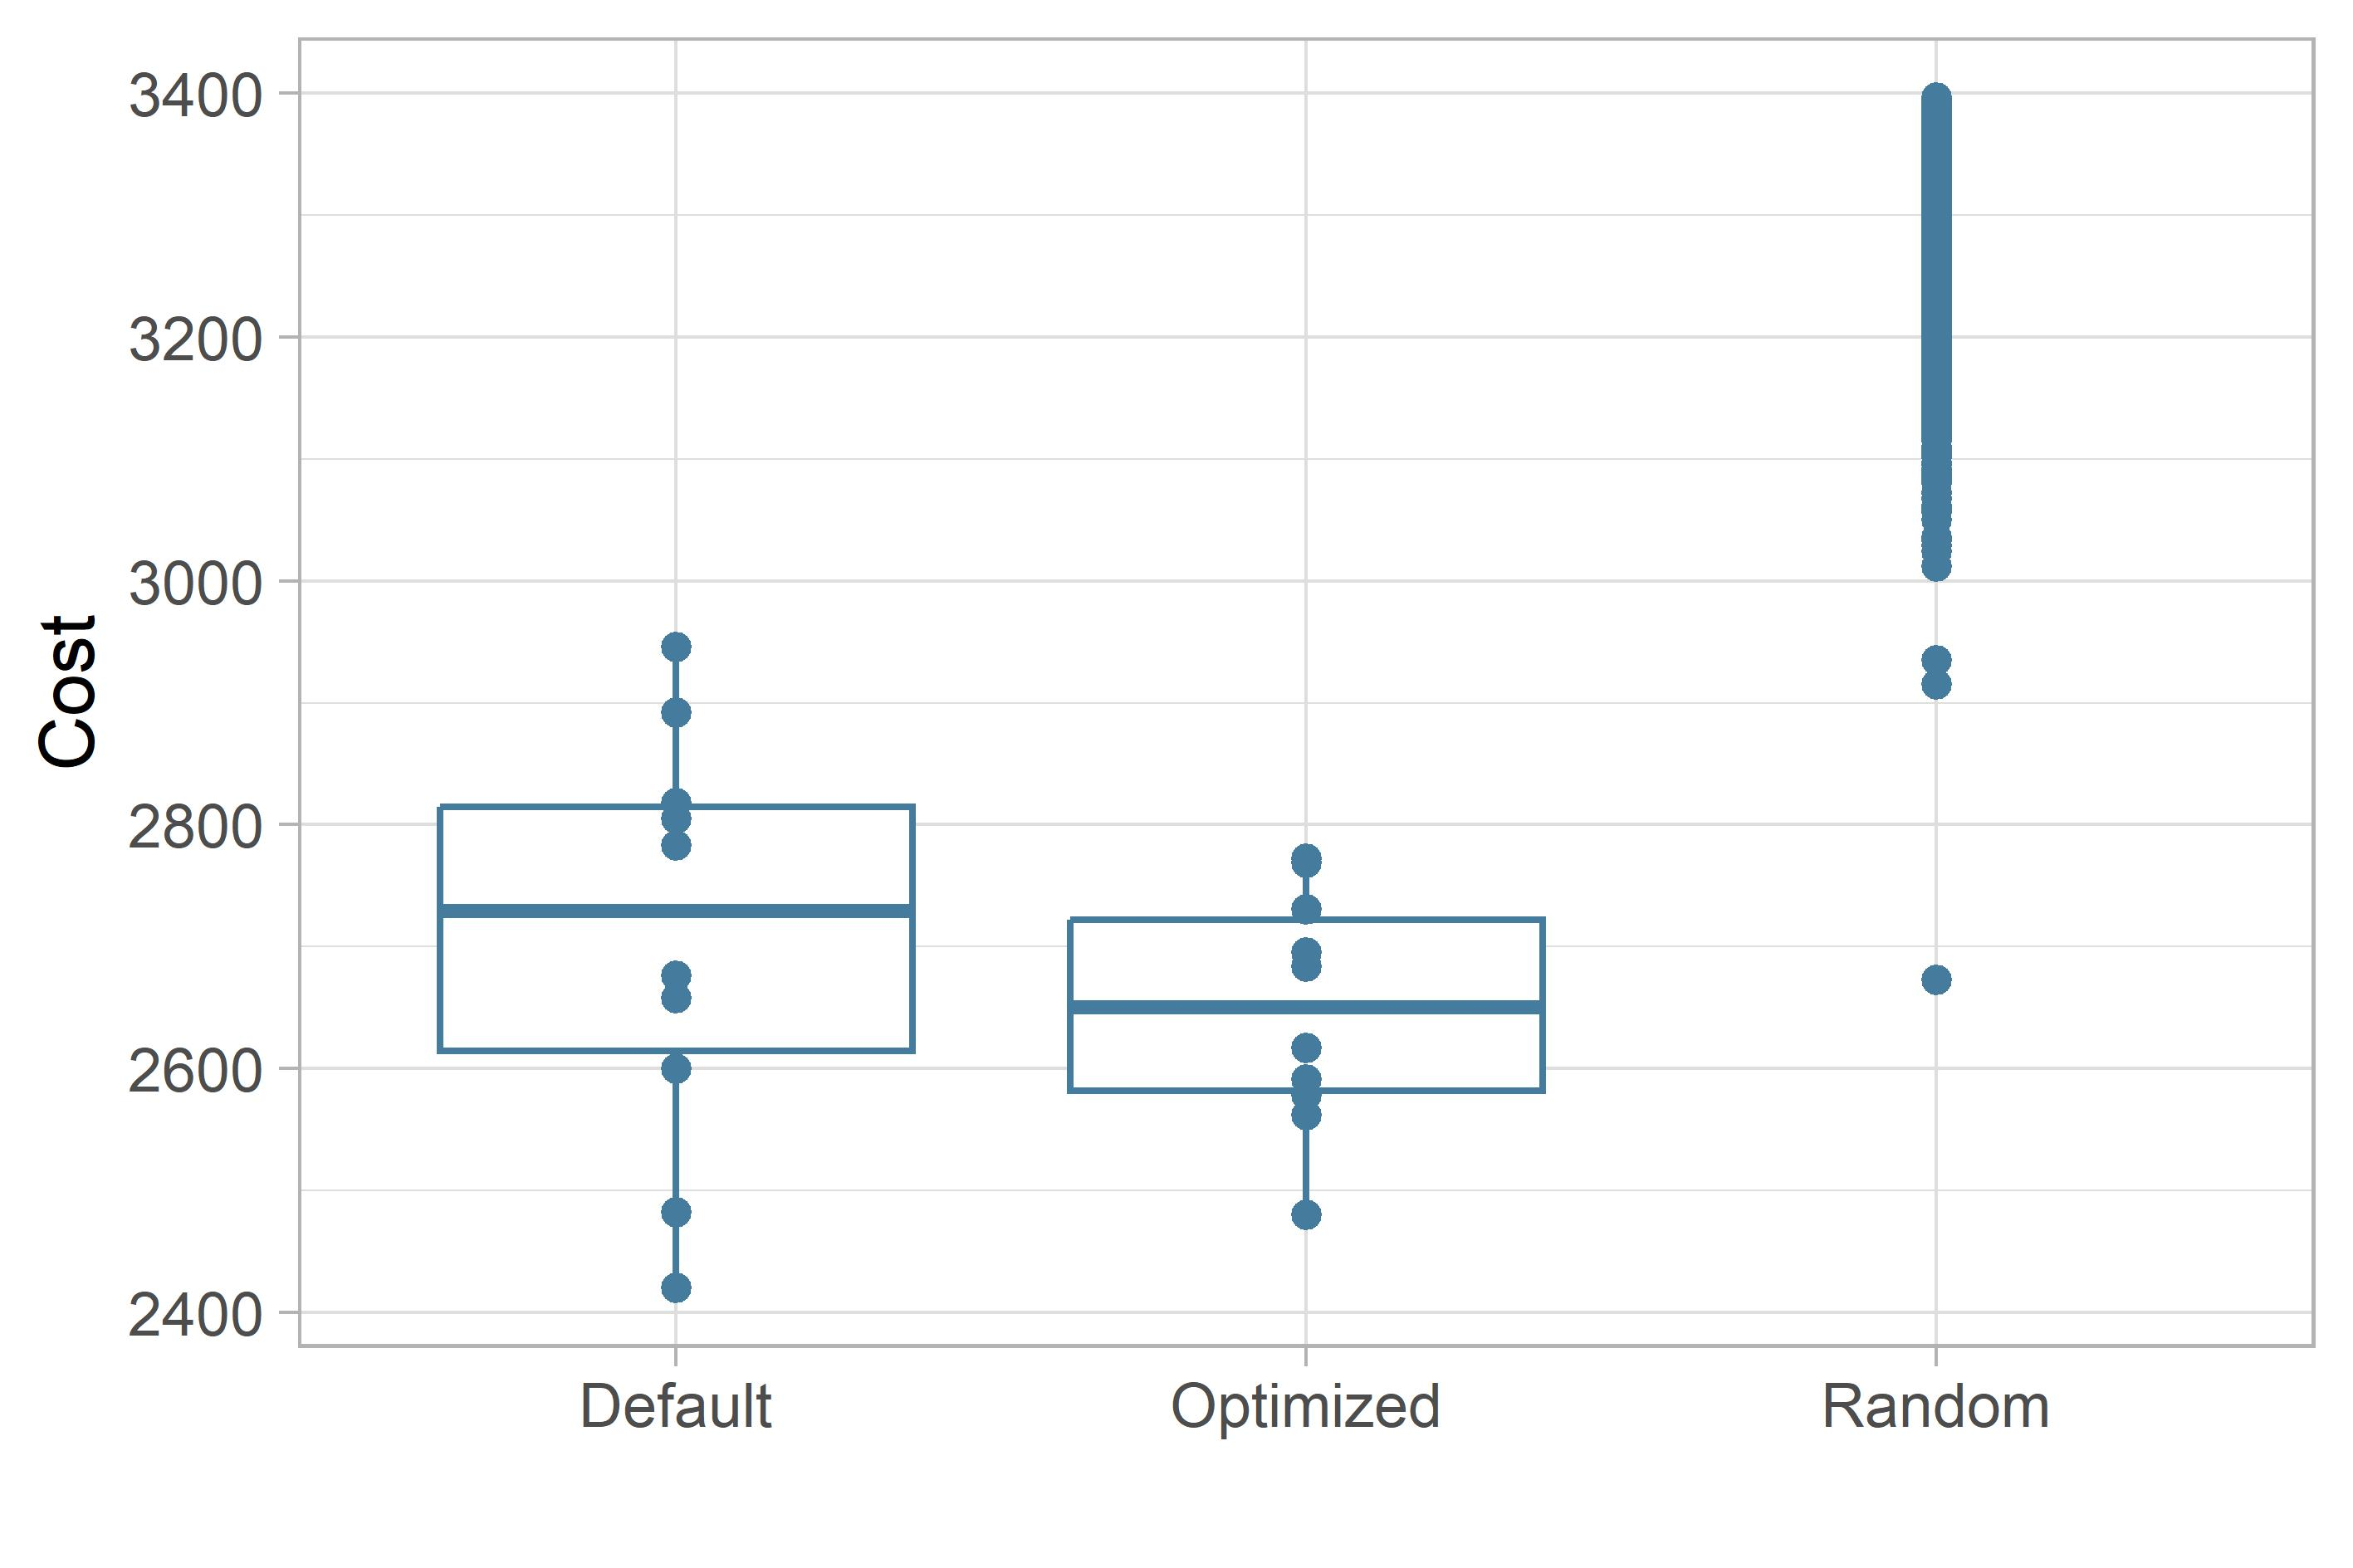
\includegraphics[width=1\linewidth]{simulations/evaluation/plots/sim_1_comparison}
	\caption{start scenario 1: Default GA vs Optimized GA vs Random Search}
	\label{fig:evaluation:sim_1_comparison}
\end{figure}

Analysing the graph, the Optimized GA clearly outperformed the Default GA as well as Random Search. Welch's t-test shows that, on average, greater fitness is achieved by using Optimized GA (M = 8.52, SE = 0.31) than by using Default GA (M = 7.09, SE = 0.34). This difference was significant \textit{t}(17.87) = 3.15, p < 0.01. It did represent a large effect r = 0.60. Compared to Random Search (M = 4.943, SE = 0.4), the Optimized GA exhibits even higher performance, with a significant difference \textit{t}(16.9) = 7.12, p < 0.001 and a large effect r = 0.87. The better performance of the Optimized GA was however unsurprising, as it was specifically trained on the used start scenario.

To further analyse both genetic algorithms, a look at their performance over the generations next to their diversity chart is of interest. Figure \ref{fig:evaluation:sim_1_ga_comparison} plots the mean over 10 repetitions, the outlines show the first and third quantiles.

\begin{figure}[ht] 
	\begin{minipage}[b]{0.5\linewidth}
		\centering
		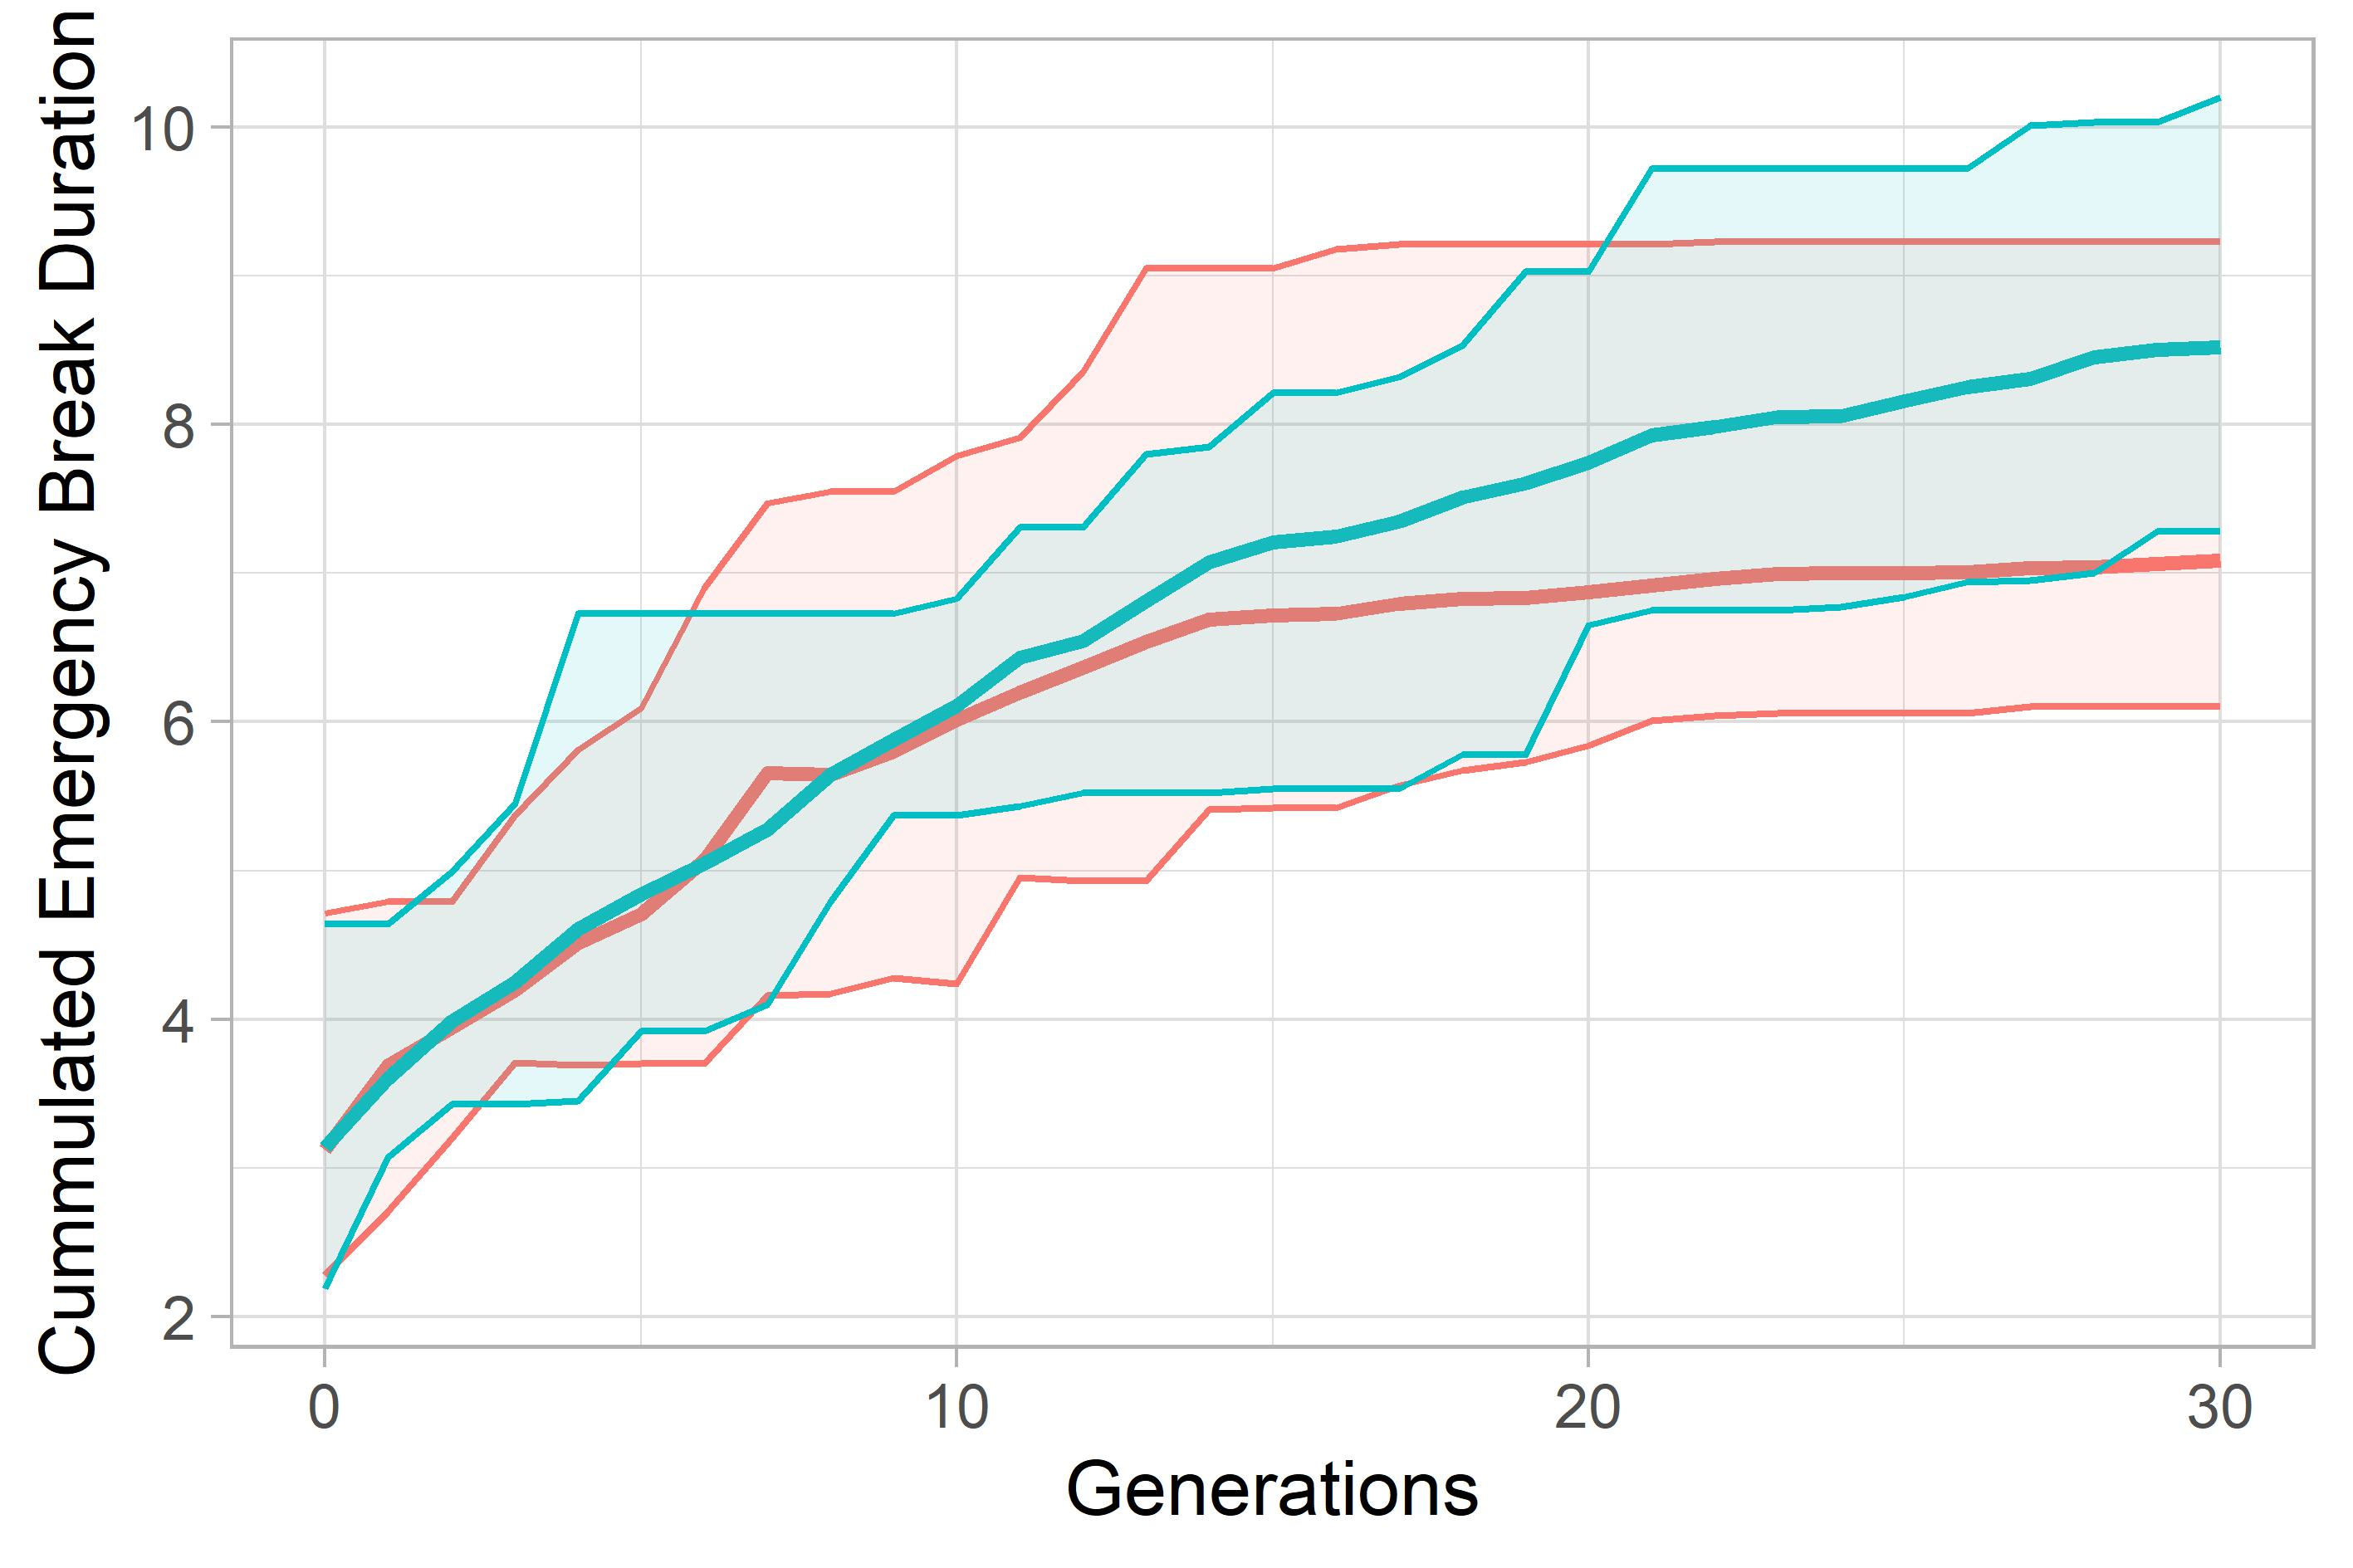
\includegraphics[width=1\linewidth]{simulations/evaluation/plots/sim_1_ga_generations} 
	\end{minipage}%%
	\begin{minipage}[b]{0.5\linewidth}
		\centering
		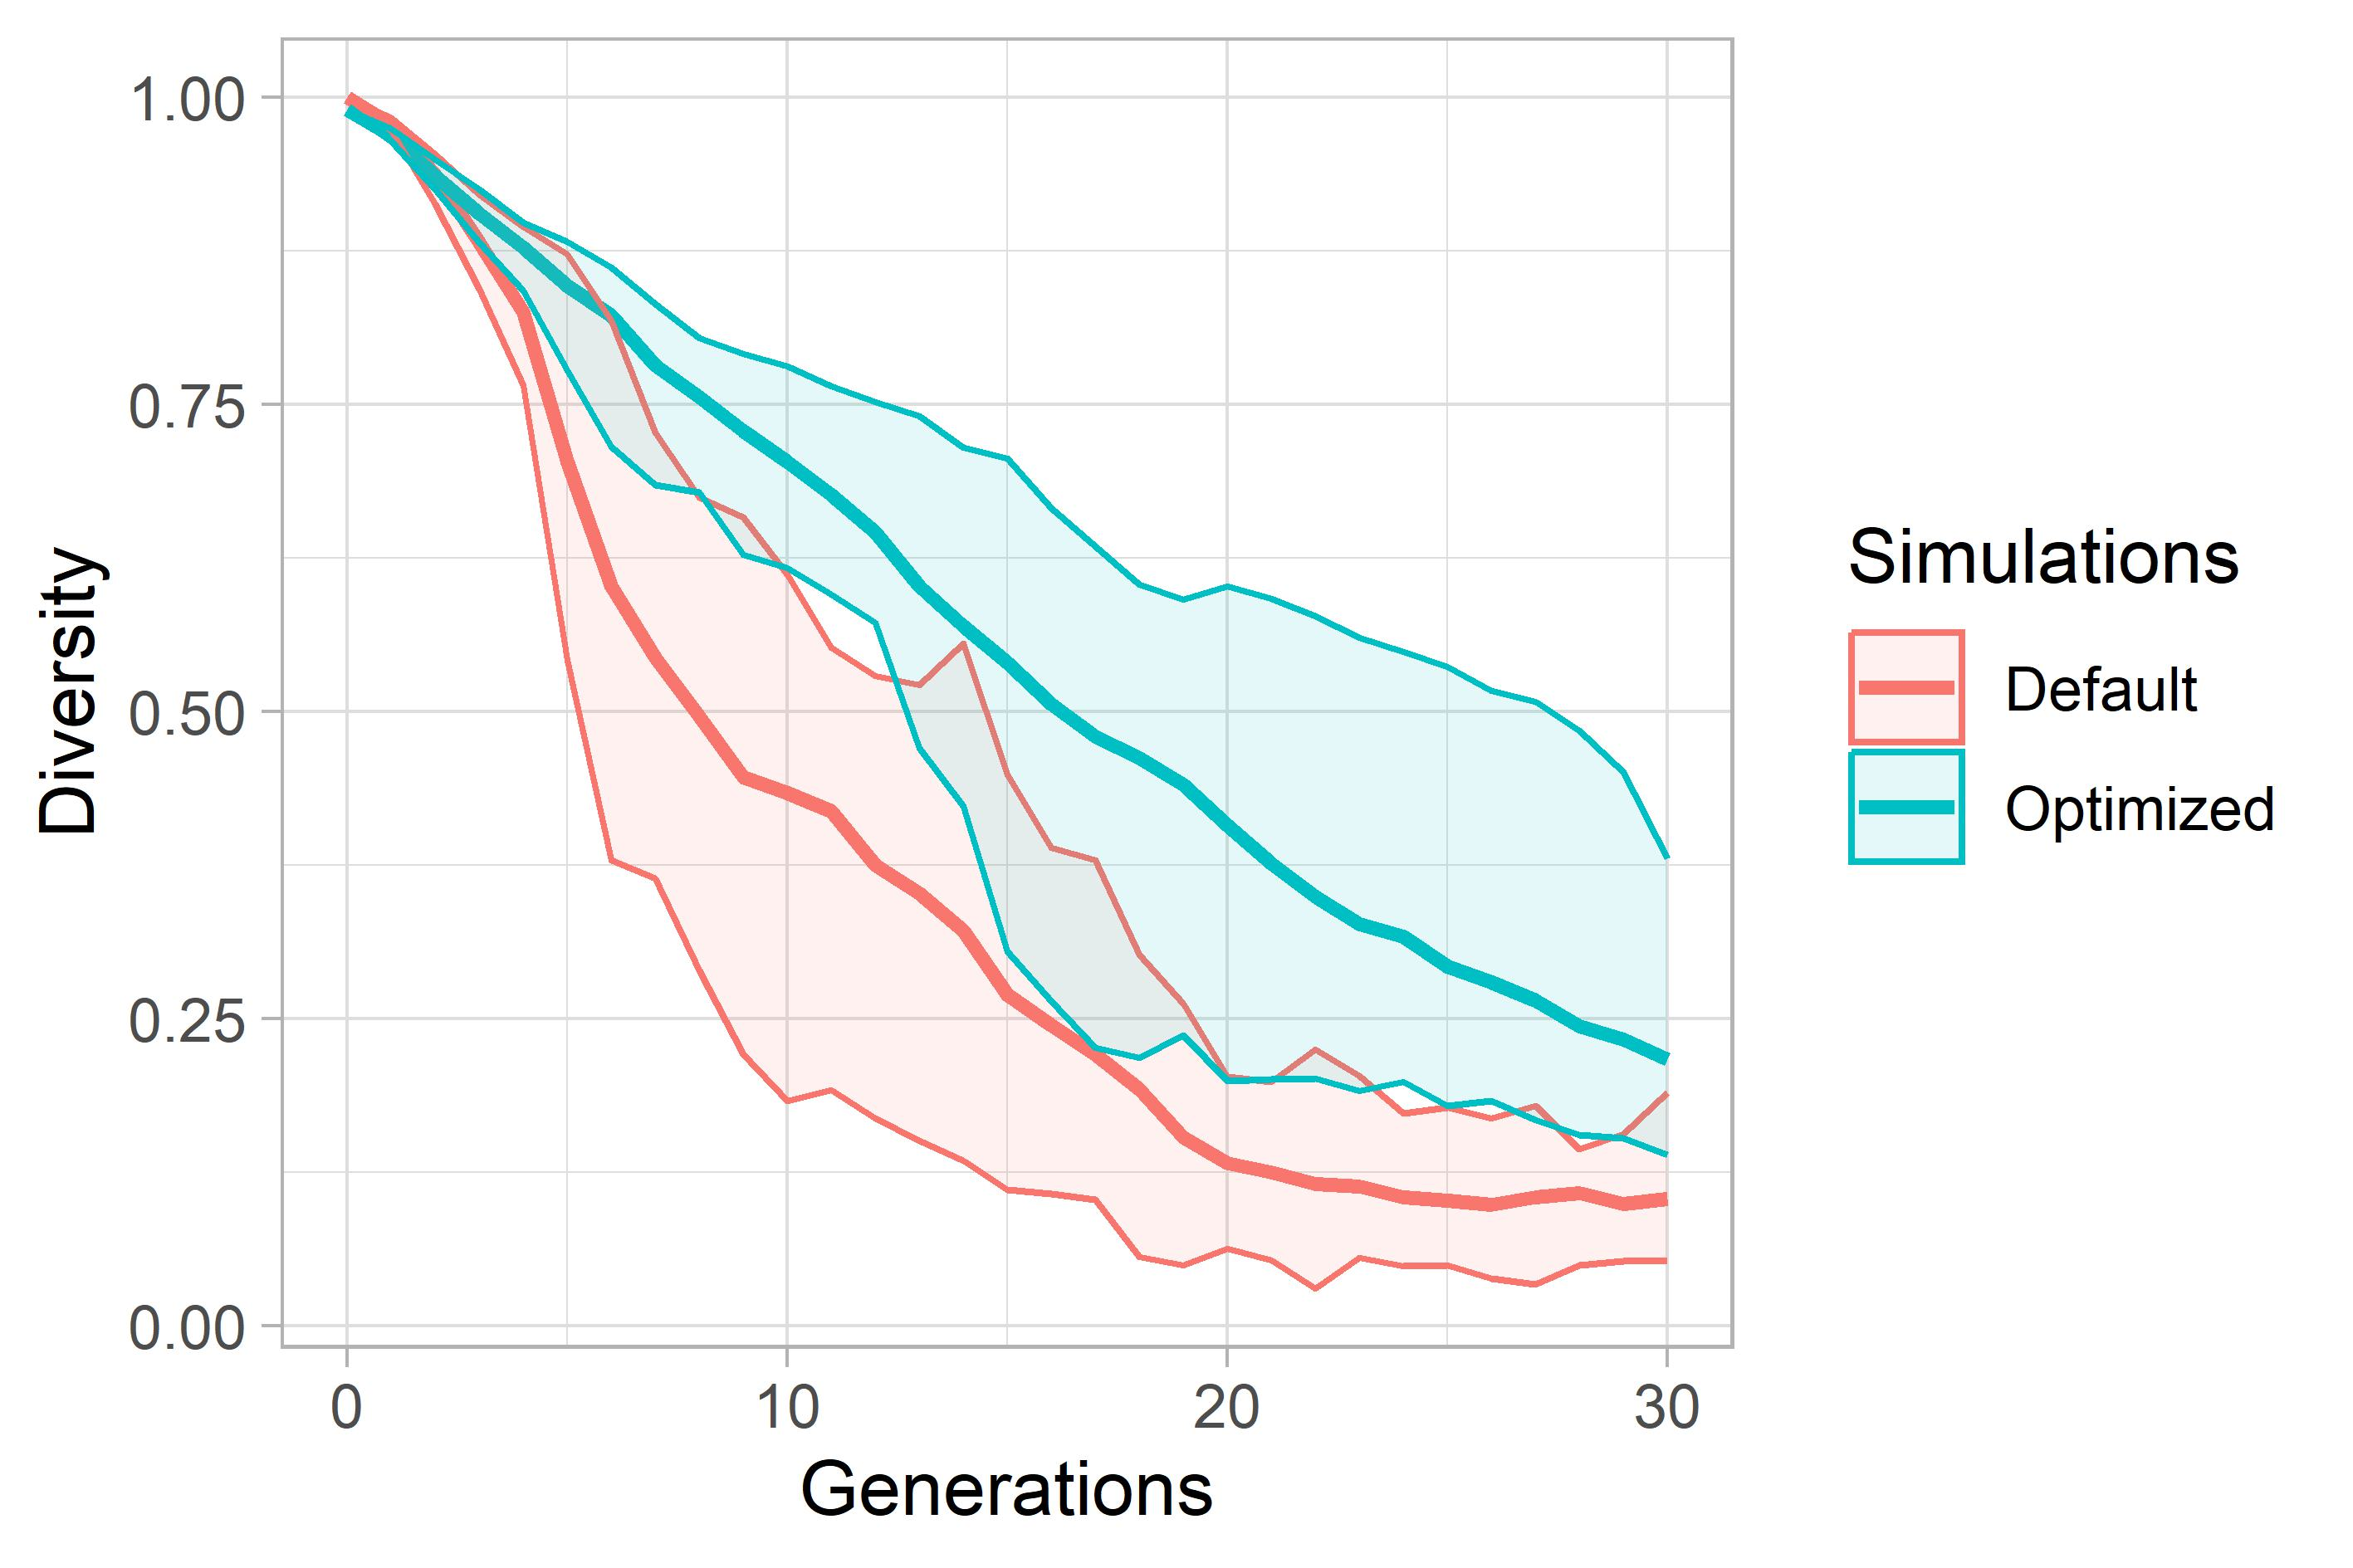
\includegraphics[width=1\linewidth]{simulations/evaluation/plots/sim_1_ga_diversity} 
	\end{minipage} 
	\caption{start scenario 1: comparison of GAs}
	\label{fig:evaluation:sim_1_ga_comparison}
\end{figure}

After generation 10, the rate of improved fitness of the Default GA decreases compared to the Optimized GA. A combined early sharp decline in the diversity, suggests a connection. The Optimized GA shows to hold the diversity in the population longer, its rate of convergence is linear. The high crossover and mutation rates appear to help with the improved diversity. The graph also shows, that a higher number of generations might not be useful for improved performance, as after 30 generations, the Optimized GA does not seem to hold enough diversity to continue with adequate performance gains. 

\section{Start Scenario 2}
Start scenario 2 has nine vehicles and five pedestrians, which is the same amount of NPCs as start scenario 1 and is described in more detail in the Appendix at Figure \ref{fig:appendix:start_scenarios_1_2}.

\begin{figure}[ht] 
	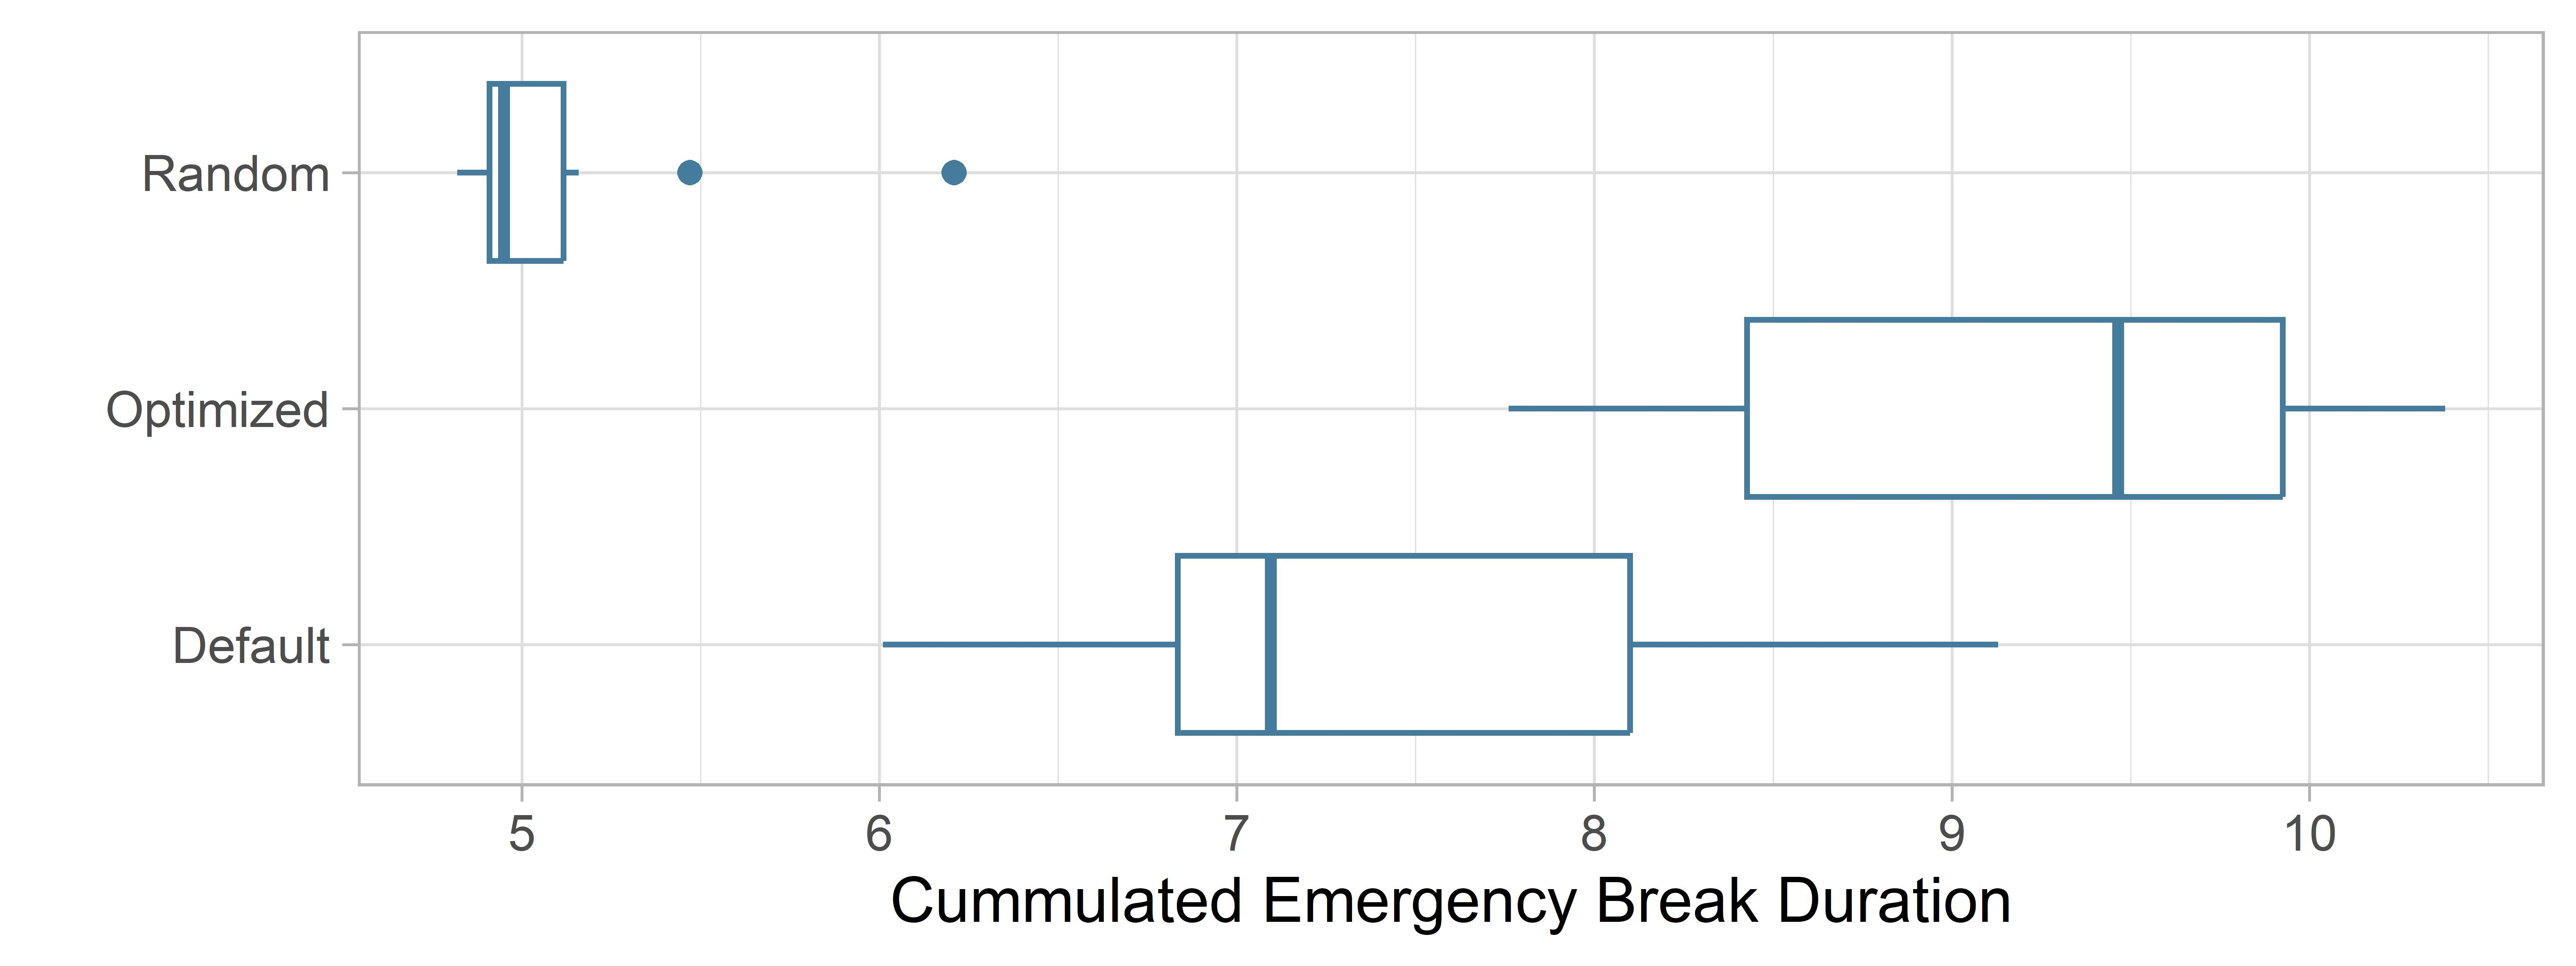
\includegraphics[width=1\linewidth]{simulations/evaluation/plots/sim_2_comparison}
	\caption{start scenario 2: Default GA vs Optimized GA vs Random Search}
	\label{fig:evaluation:sim_2_comparison}
\end{figure}

Figure \ref{fig:evaluation:sim_2_comparison} shows that the Optimized GA can also provide better results compared to the other two algorithms in start scenarios where it has not be trained on. The Optimized GA (M = 9.24, SE = 0.3) achieves better fitness on average compared to the Default GA (M = 7.46, SE = 0.31, with a significant difference \textit{t}(17.98) = 4.19, p < 0.001 and a large effect of r = 0.7. The difference in the average fitness value compared Random Search (M = 5.13, SE = 0.13) is significant as well with \textit{t}(12.57) = 12.7, p < 0.001 and a large effect of r = 0.96.

\begin{figure}[ht] 
	\begin{minipage}[b]{0.5\linewidth}
		\centering
		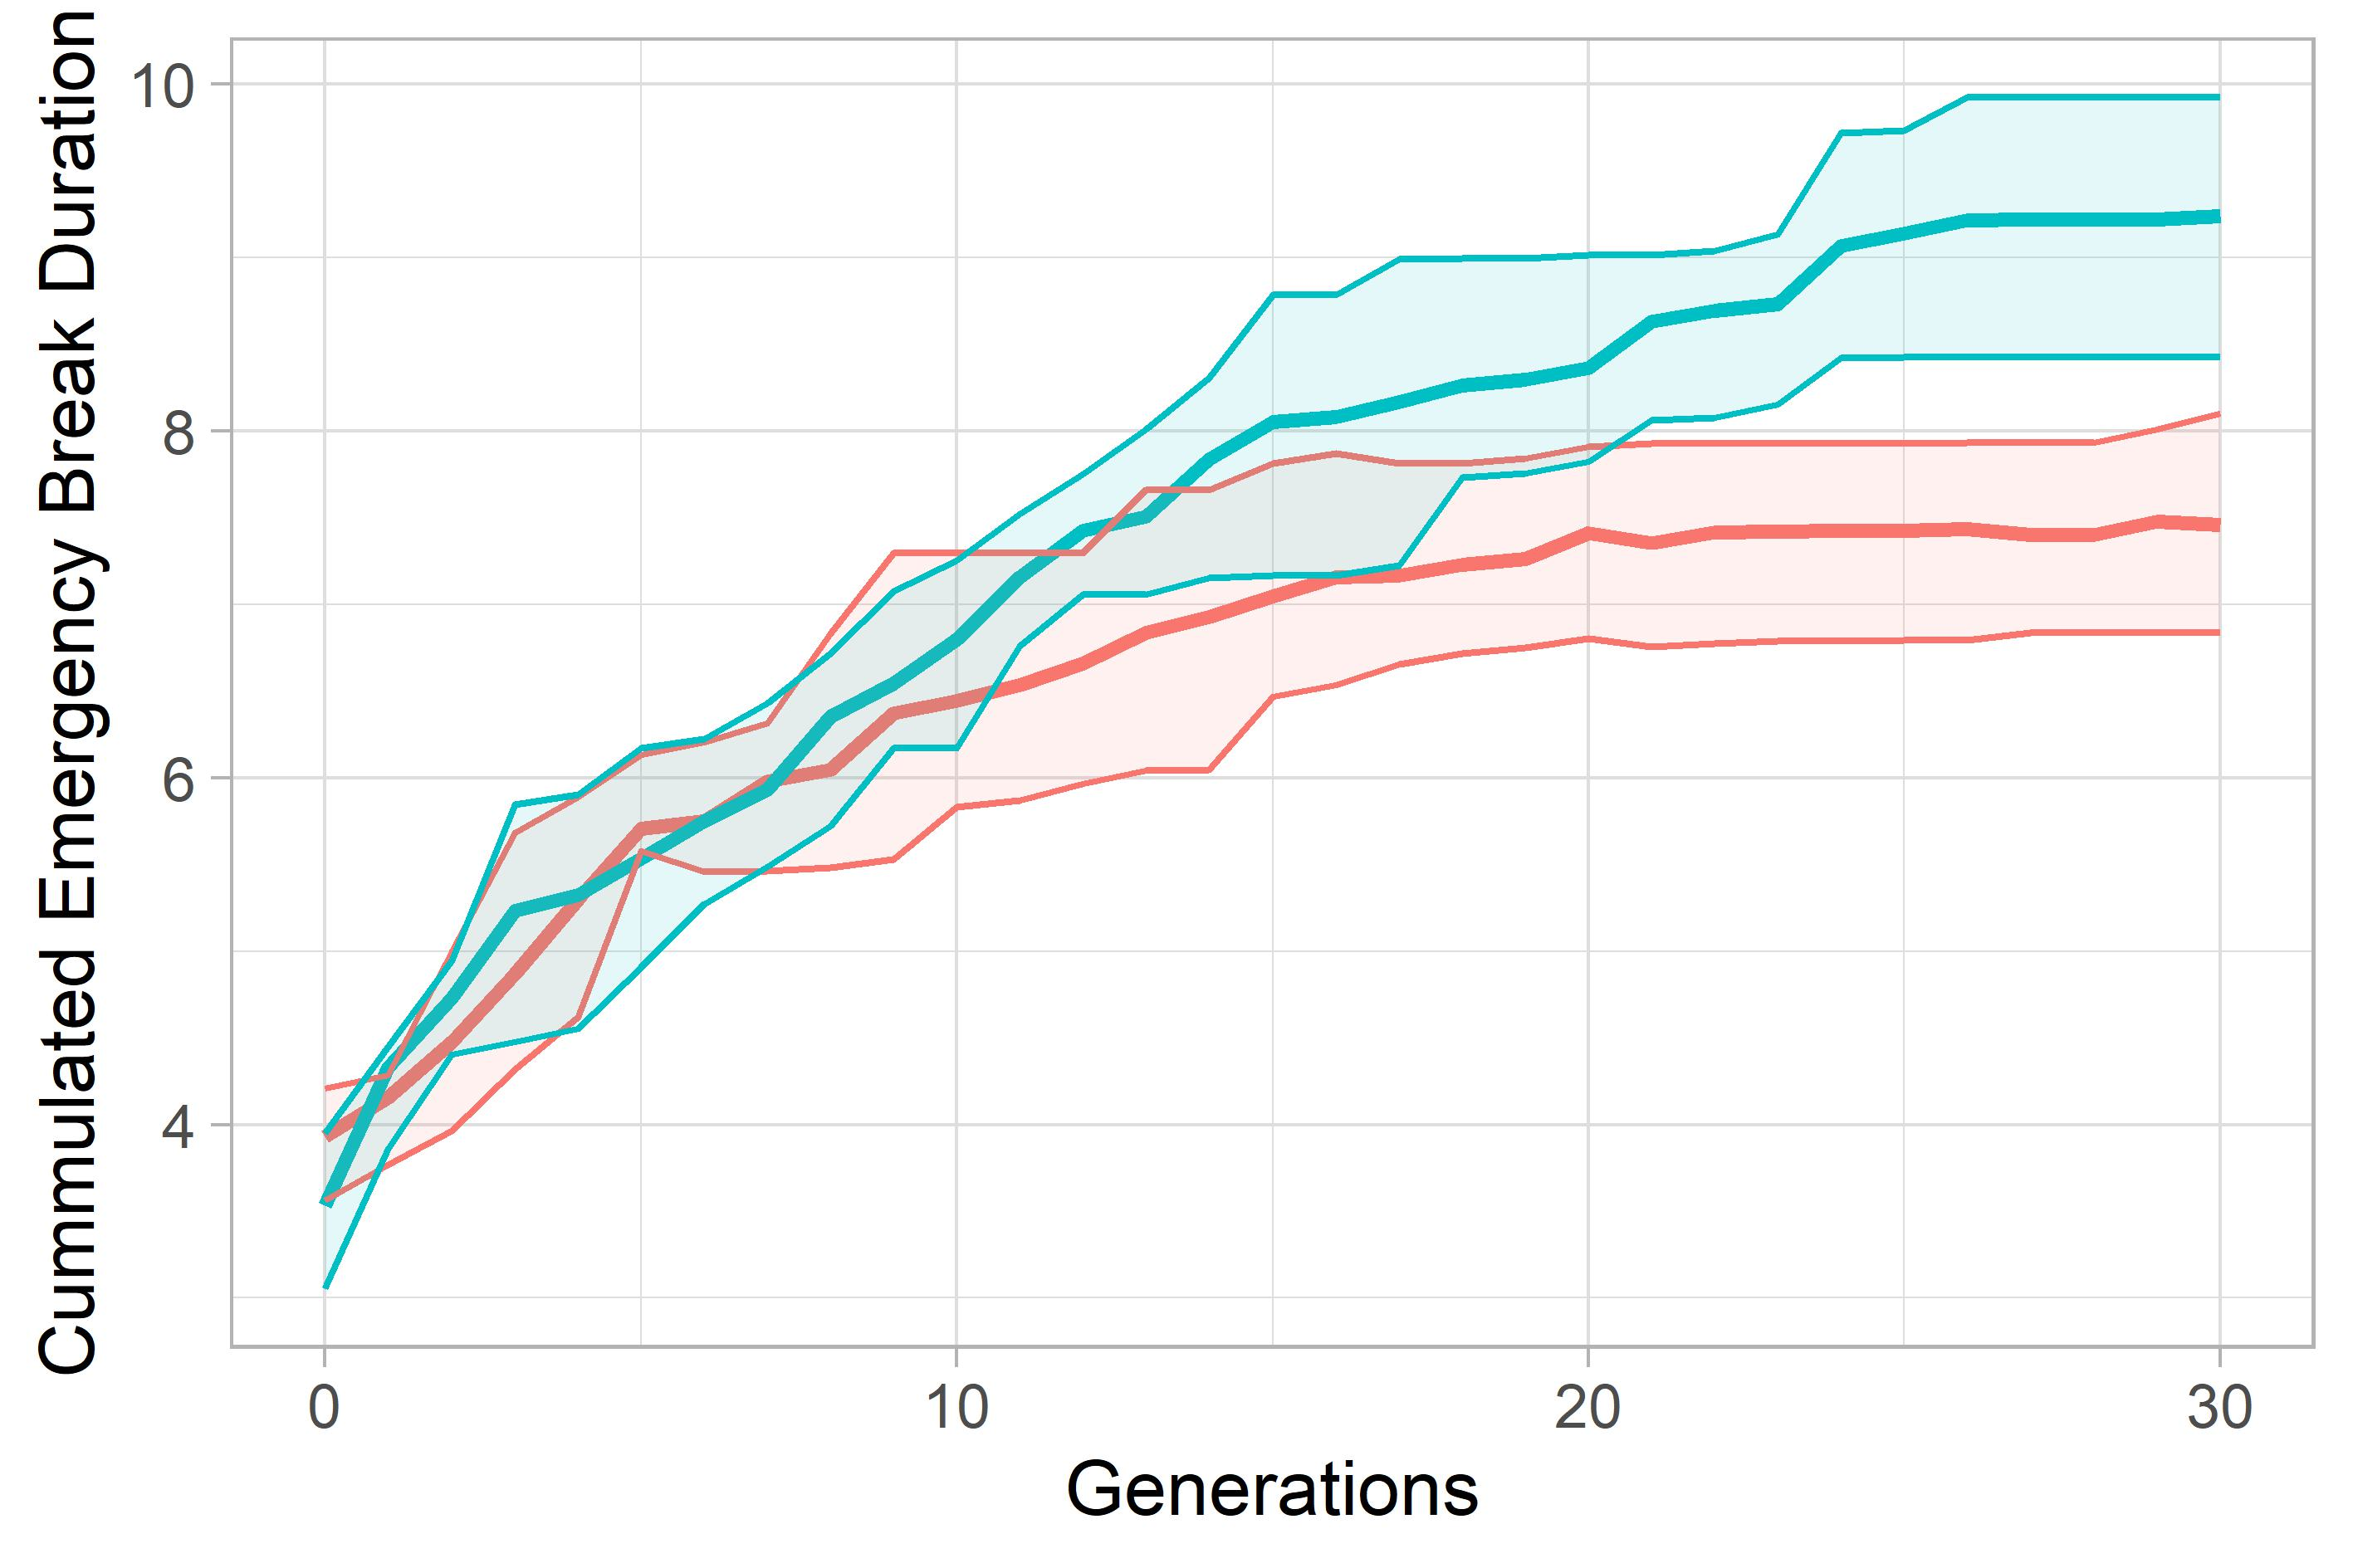
\includegraphics[width=1\linewidth]{simulations/evaluation/plots/sim_2_ga_generations} 
	\end{minipage}%%
	\begin{minipage}[b]{0.5\linewidth}
		\centering
		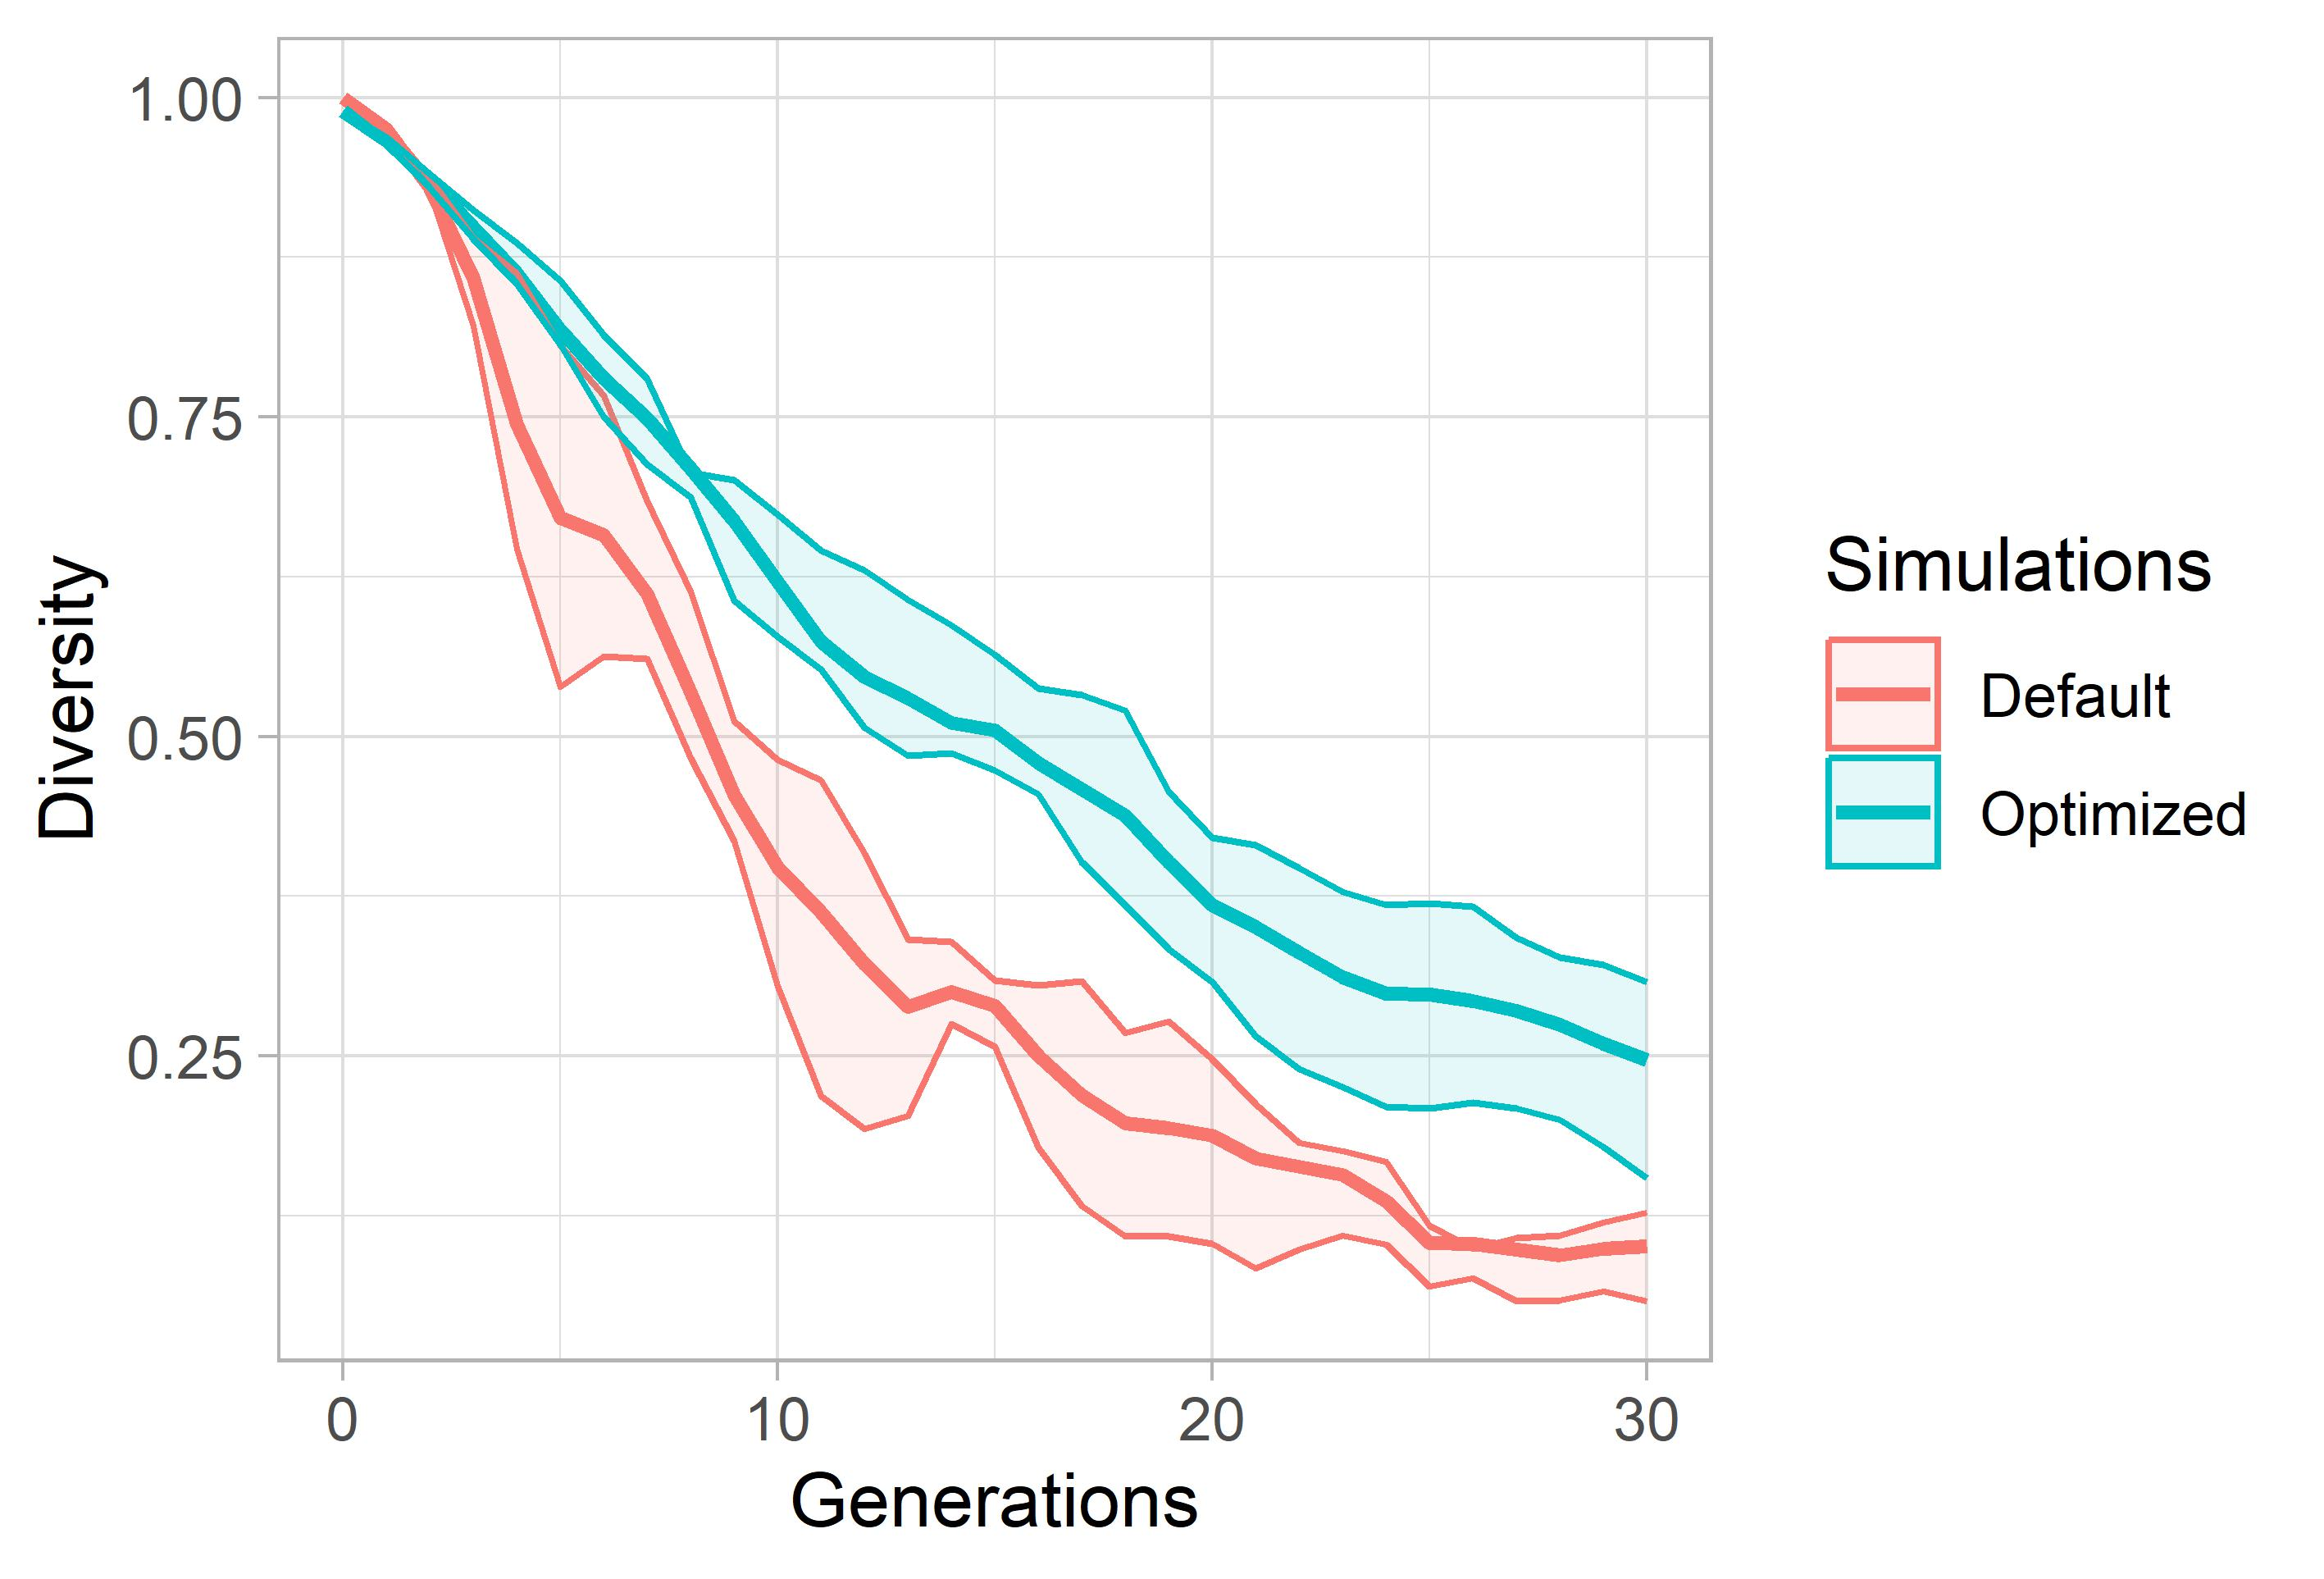
\includegraphics[width=1\linewidth]{simulations/evaluation/plots/sim_2_ga_diversity} 
	\end{minipage} 
	\caption{start scenario 2: comparison of GAs}
	\label{fig:evaluation:sim_2_ga_comparison}
\end{figure}

The comparison shown in Figure \ref{fig:evaluation:sim_2_ga_comparison} seems very similar to the comparison discussed in start scenario 1. While the Default GA again shows to not be able to keep up with the high performance increase of the Optimized GA, the diversity of the Optimized GA drops a bit sooner compared to previously. Still both evaluations show, that the Optimized GA performs well in start scenarios with the given amount of NPCs.

\section{Start Scenario 3}
\label{sect:evaluation:scenario_3}
Start scenario 3 is described in more detail in Appendix at Figure \ref{fig:appendix:start_scenarios_3_4}. Five vehicles with three pedestrians are initialized, resulting in a simulation with only a small number of NPCs.

\begin{figure}[ht] 
	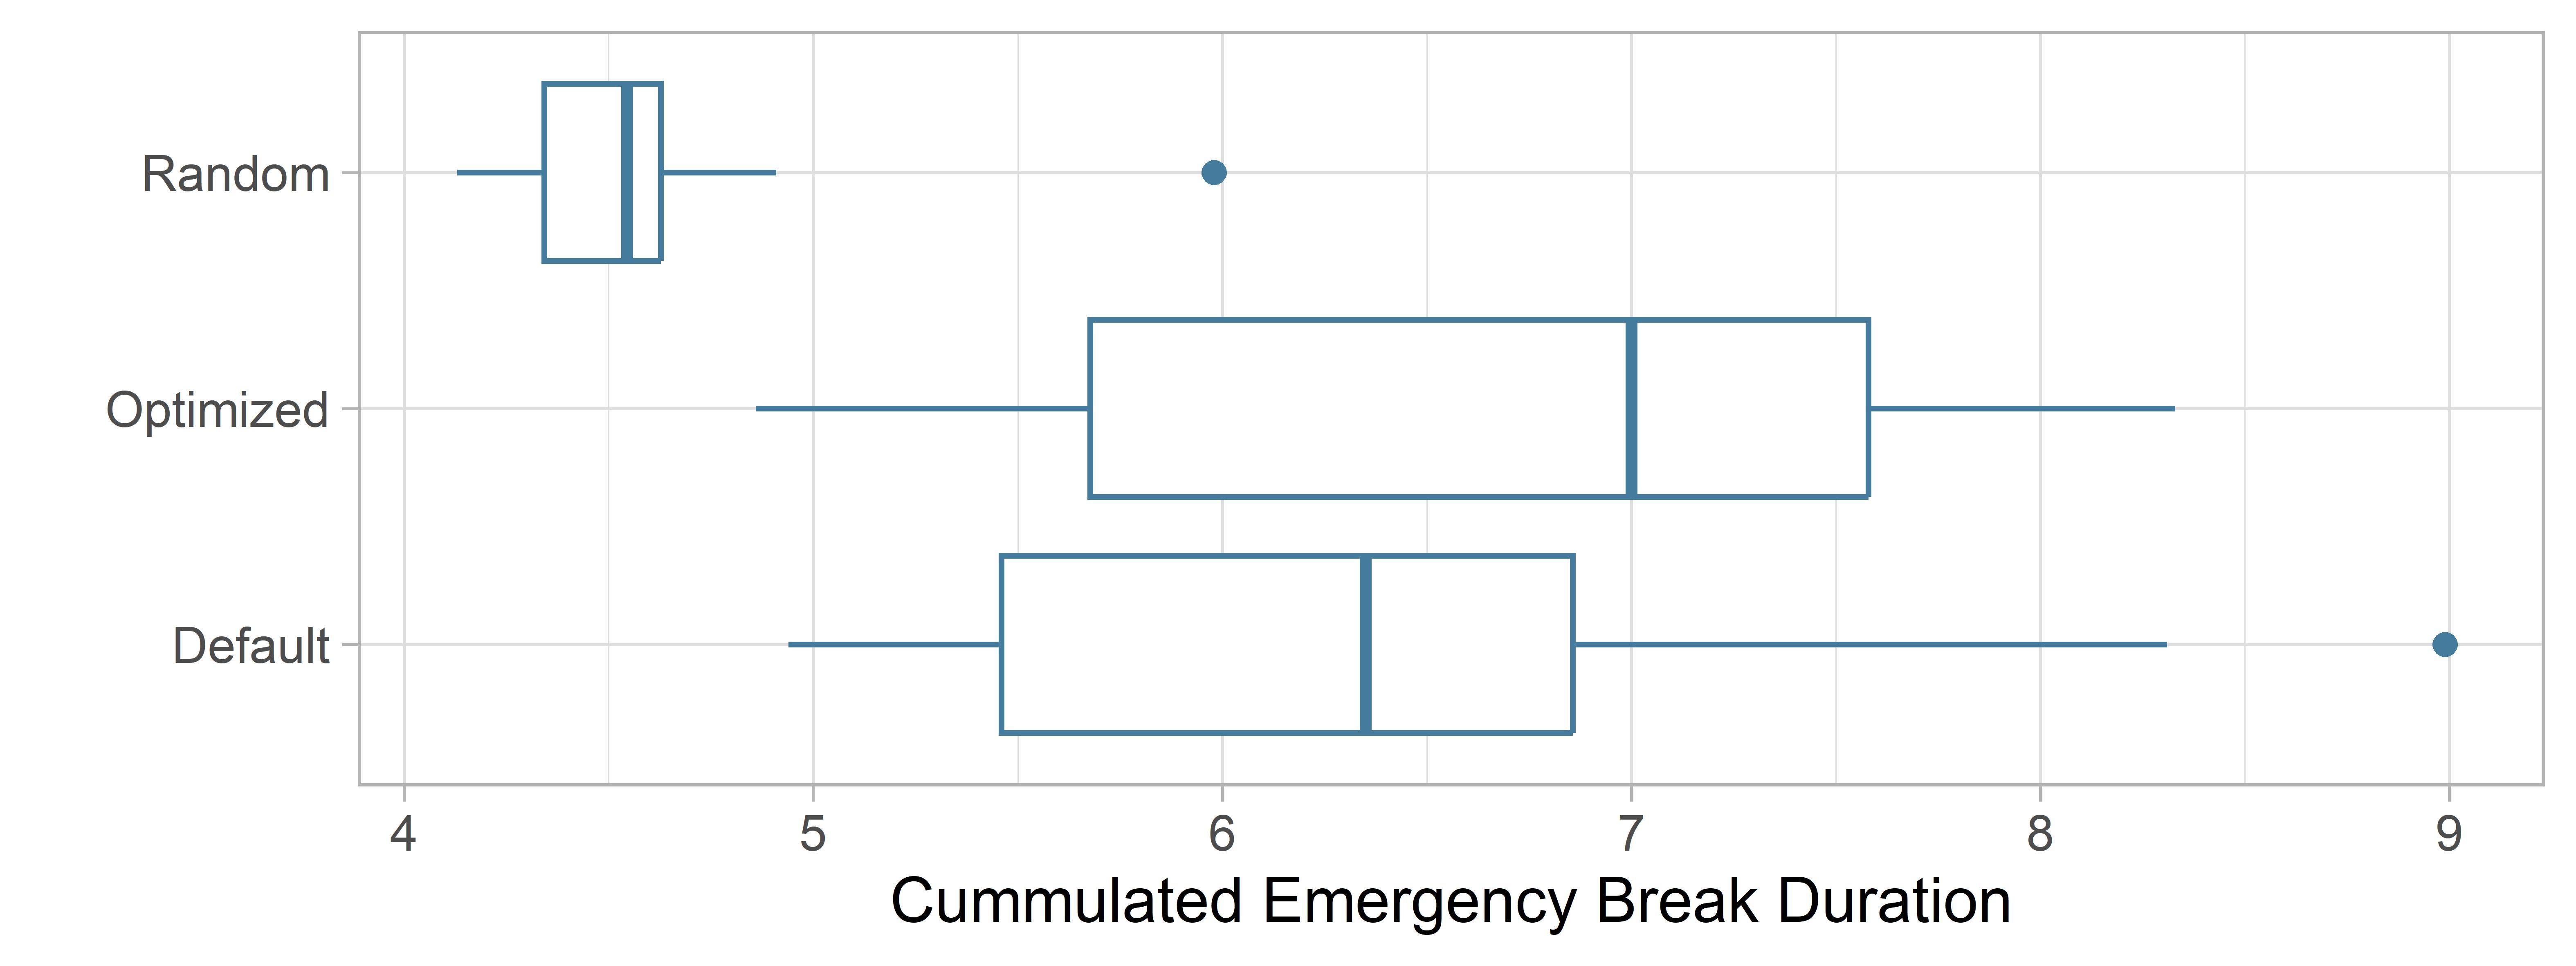
\includegraphics[width=1\linewidth]{simulations/evaluation/plots/sim_3_comparison}
	\caption{start scenario 3: Default GA vs Optimized GA vs Random Search}
	\label{fig:evaluation:sim_3_comparison}
\end{figure}

Looking at the graph, the Optimized GA again outperforms the Random Search, however there seems to be only marginal improvements compared to Default GA. A Welch's t-test confirms these findings. While on average, greater fitness is achieved by using Optimized GA (M = 6.66, SE = 0.38) than from using Default GA (M = 6.49, SE = 0.42), this difference was not significant \textit{t}(17.83) = 0.29, p > 0.05 with an effect size of r = 0.07. Verifying the better performance of the Optimized GA compared to Random Search (M = 4.619, SE = 0.17) shows a significant difference \textit{t}(12.4) = 4.9, p < 0.001 and a large effect size of r = 0.81. To further analyse both genetic algorithms, their performance over the generations next to their diversity chart is shown in Figure \ref{fig:evaluation:sim_3_ga_comparison}. The mean over 10 repetitions is plotted, the outline show the first and third quantiles.

\begin{figure}[ht] 
	\begin{minipage}[b]{0.5\linewidth}
		\centering
		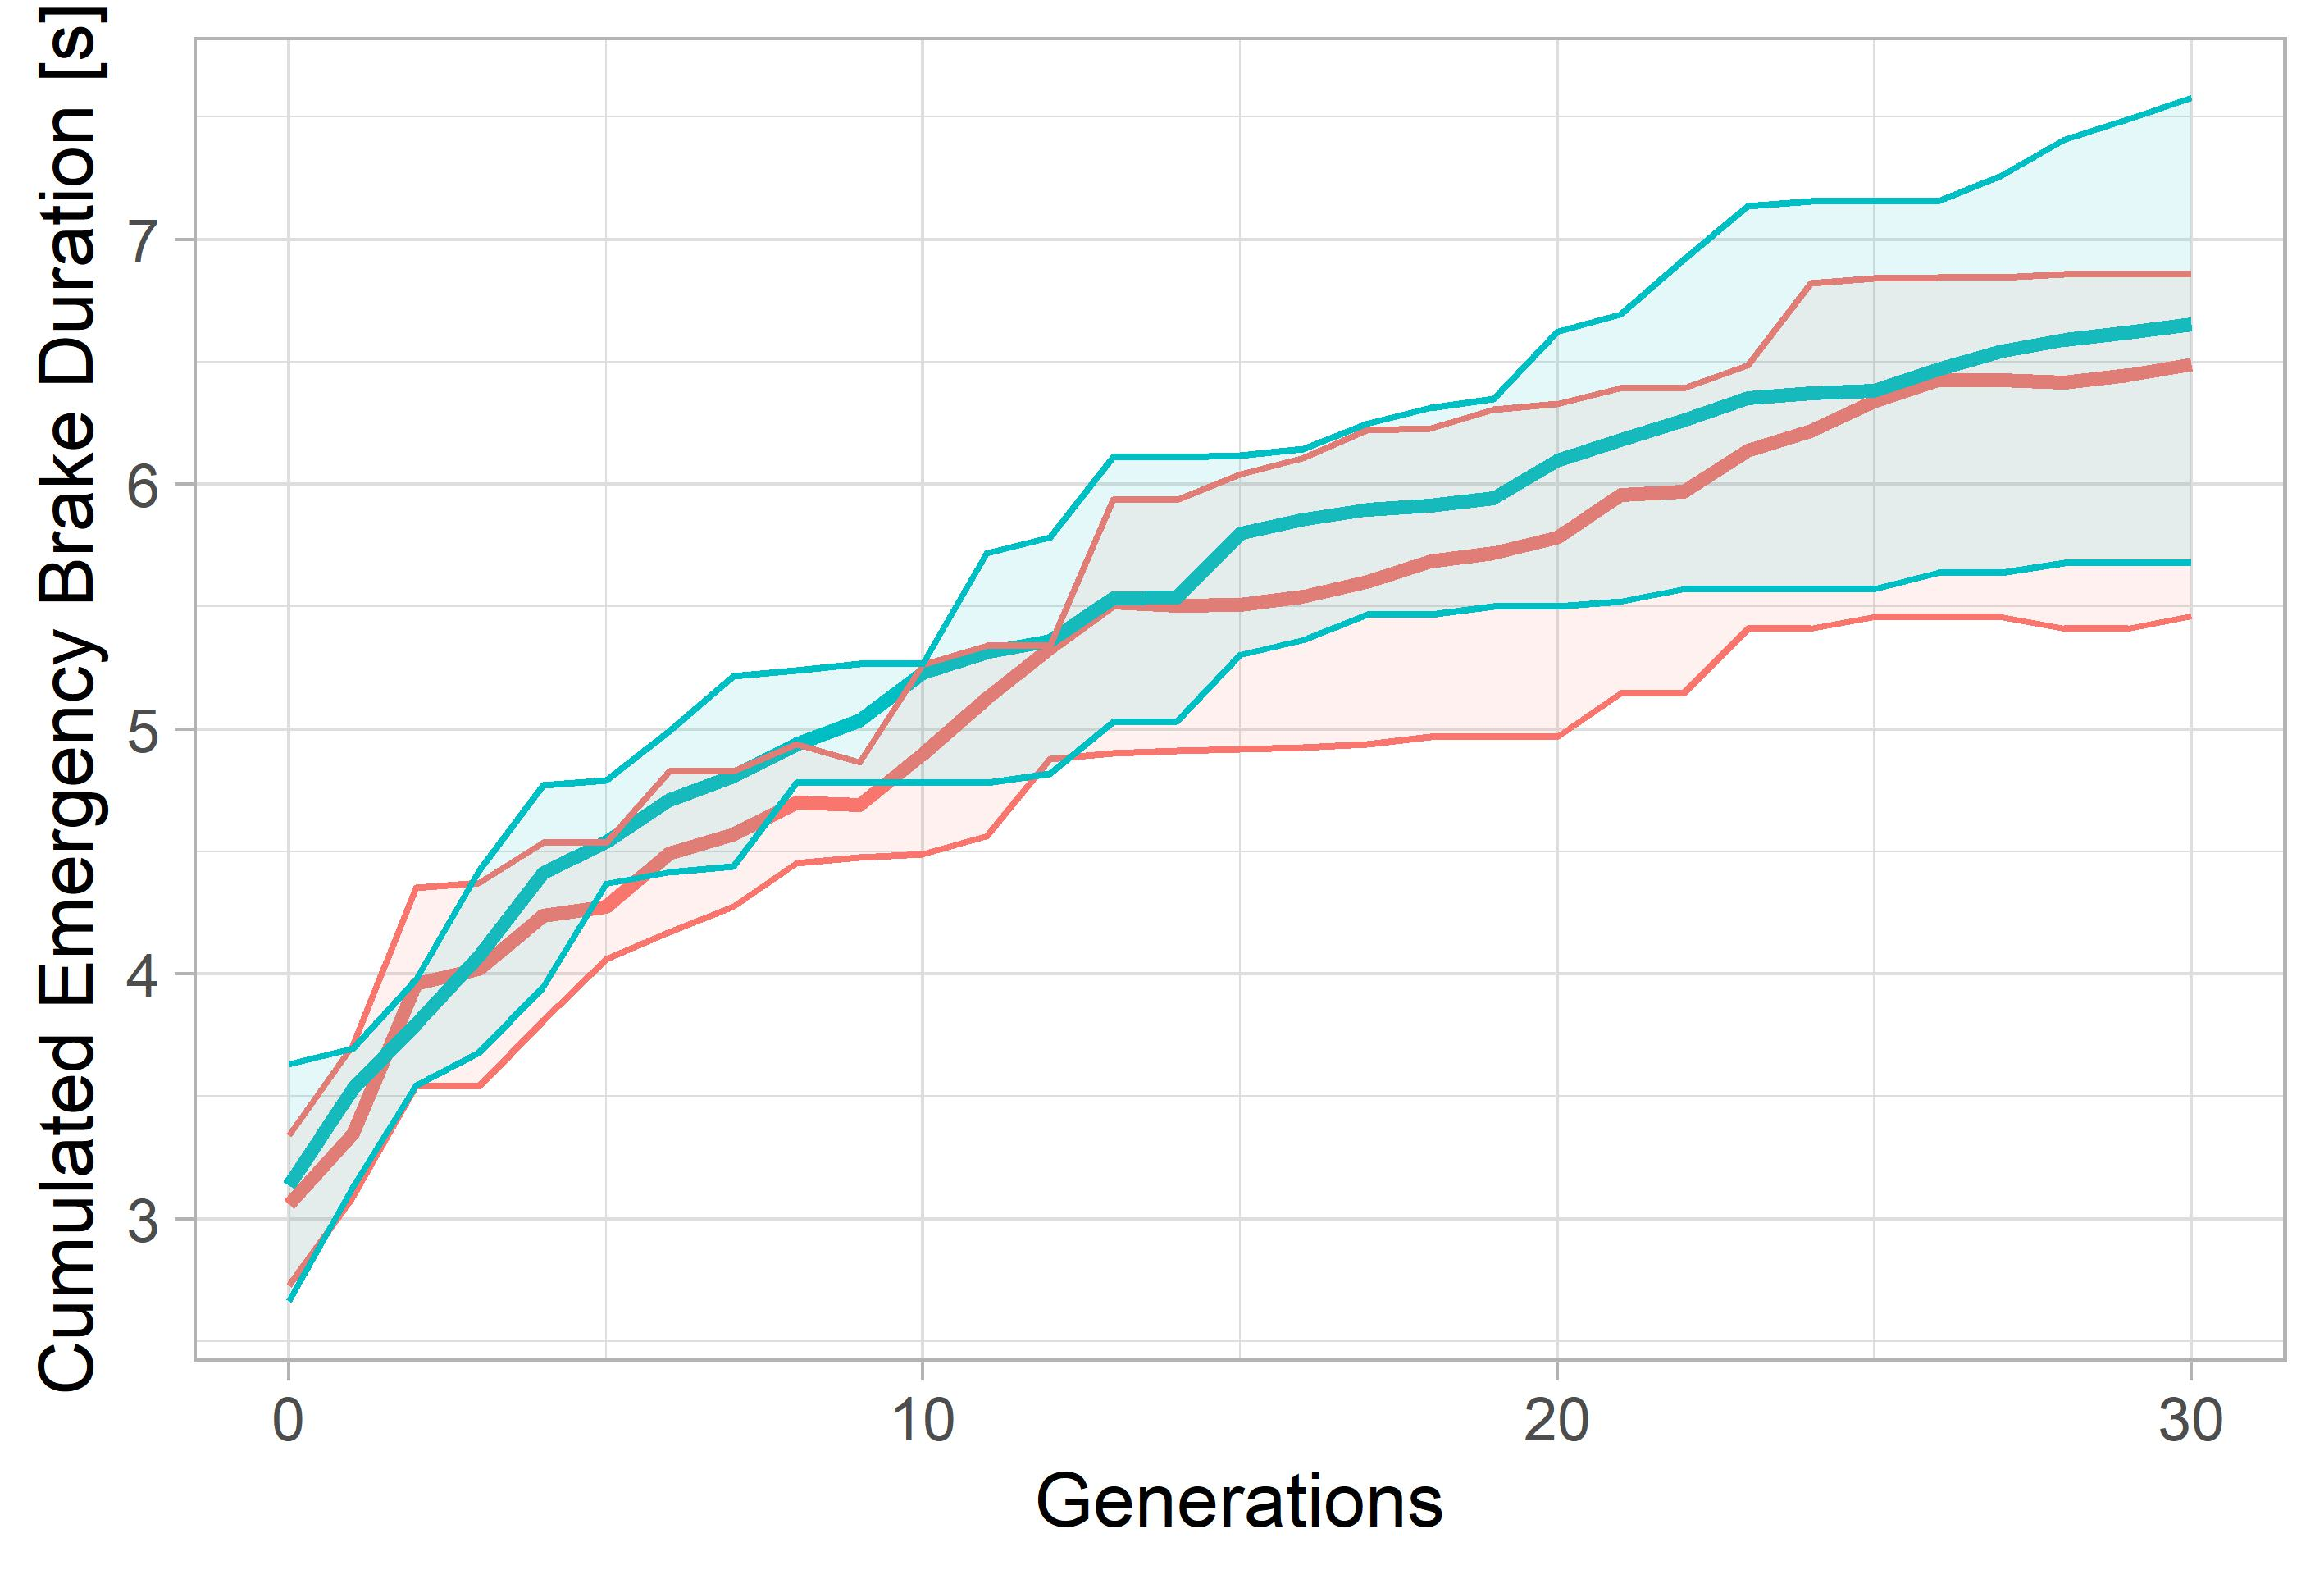
\includegraphics[width=1\linewidth]{simulations/evaluation/plots/sim_3_ga_generations} 
	\end{minipage}%%
	\begin{minipage}[b]{0.5\linewidth}
		\centering
		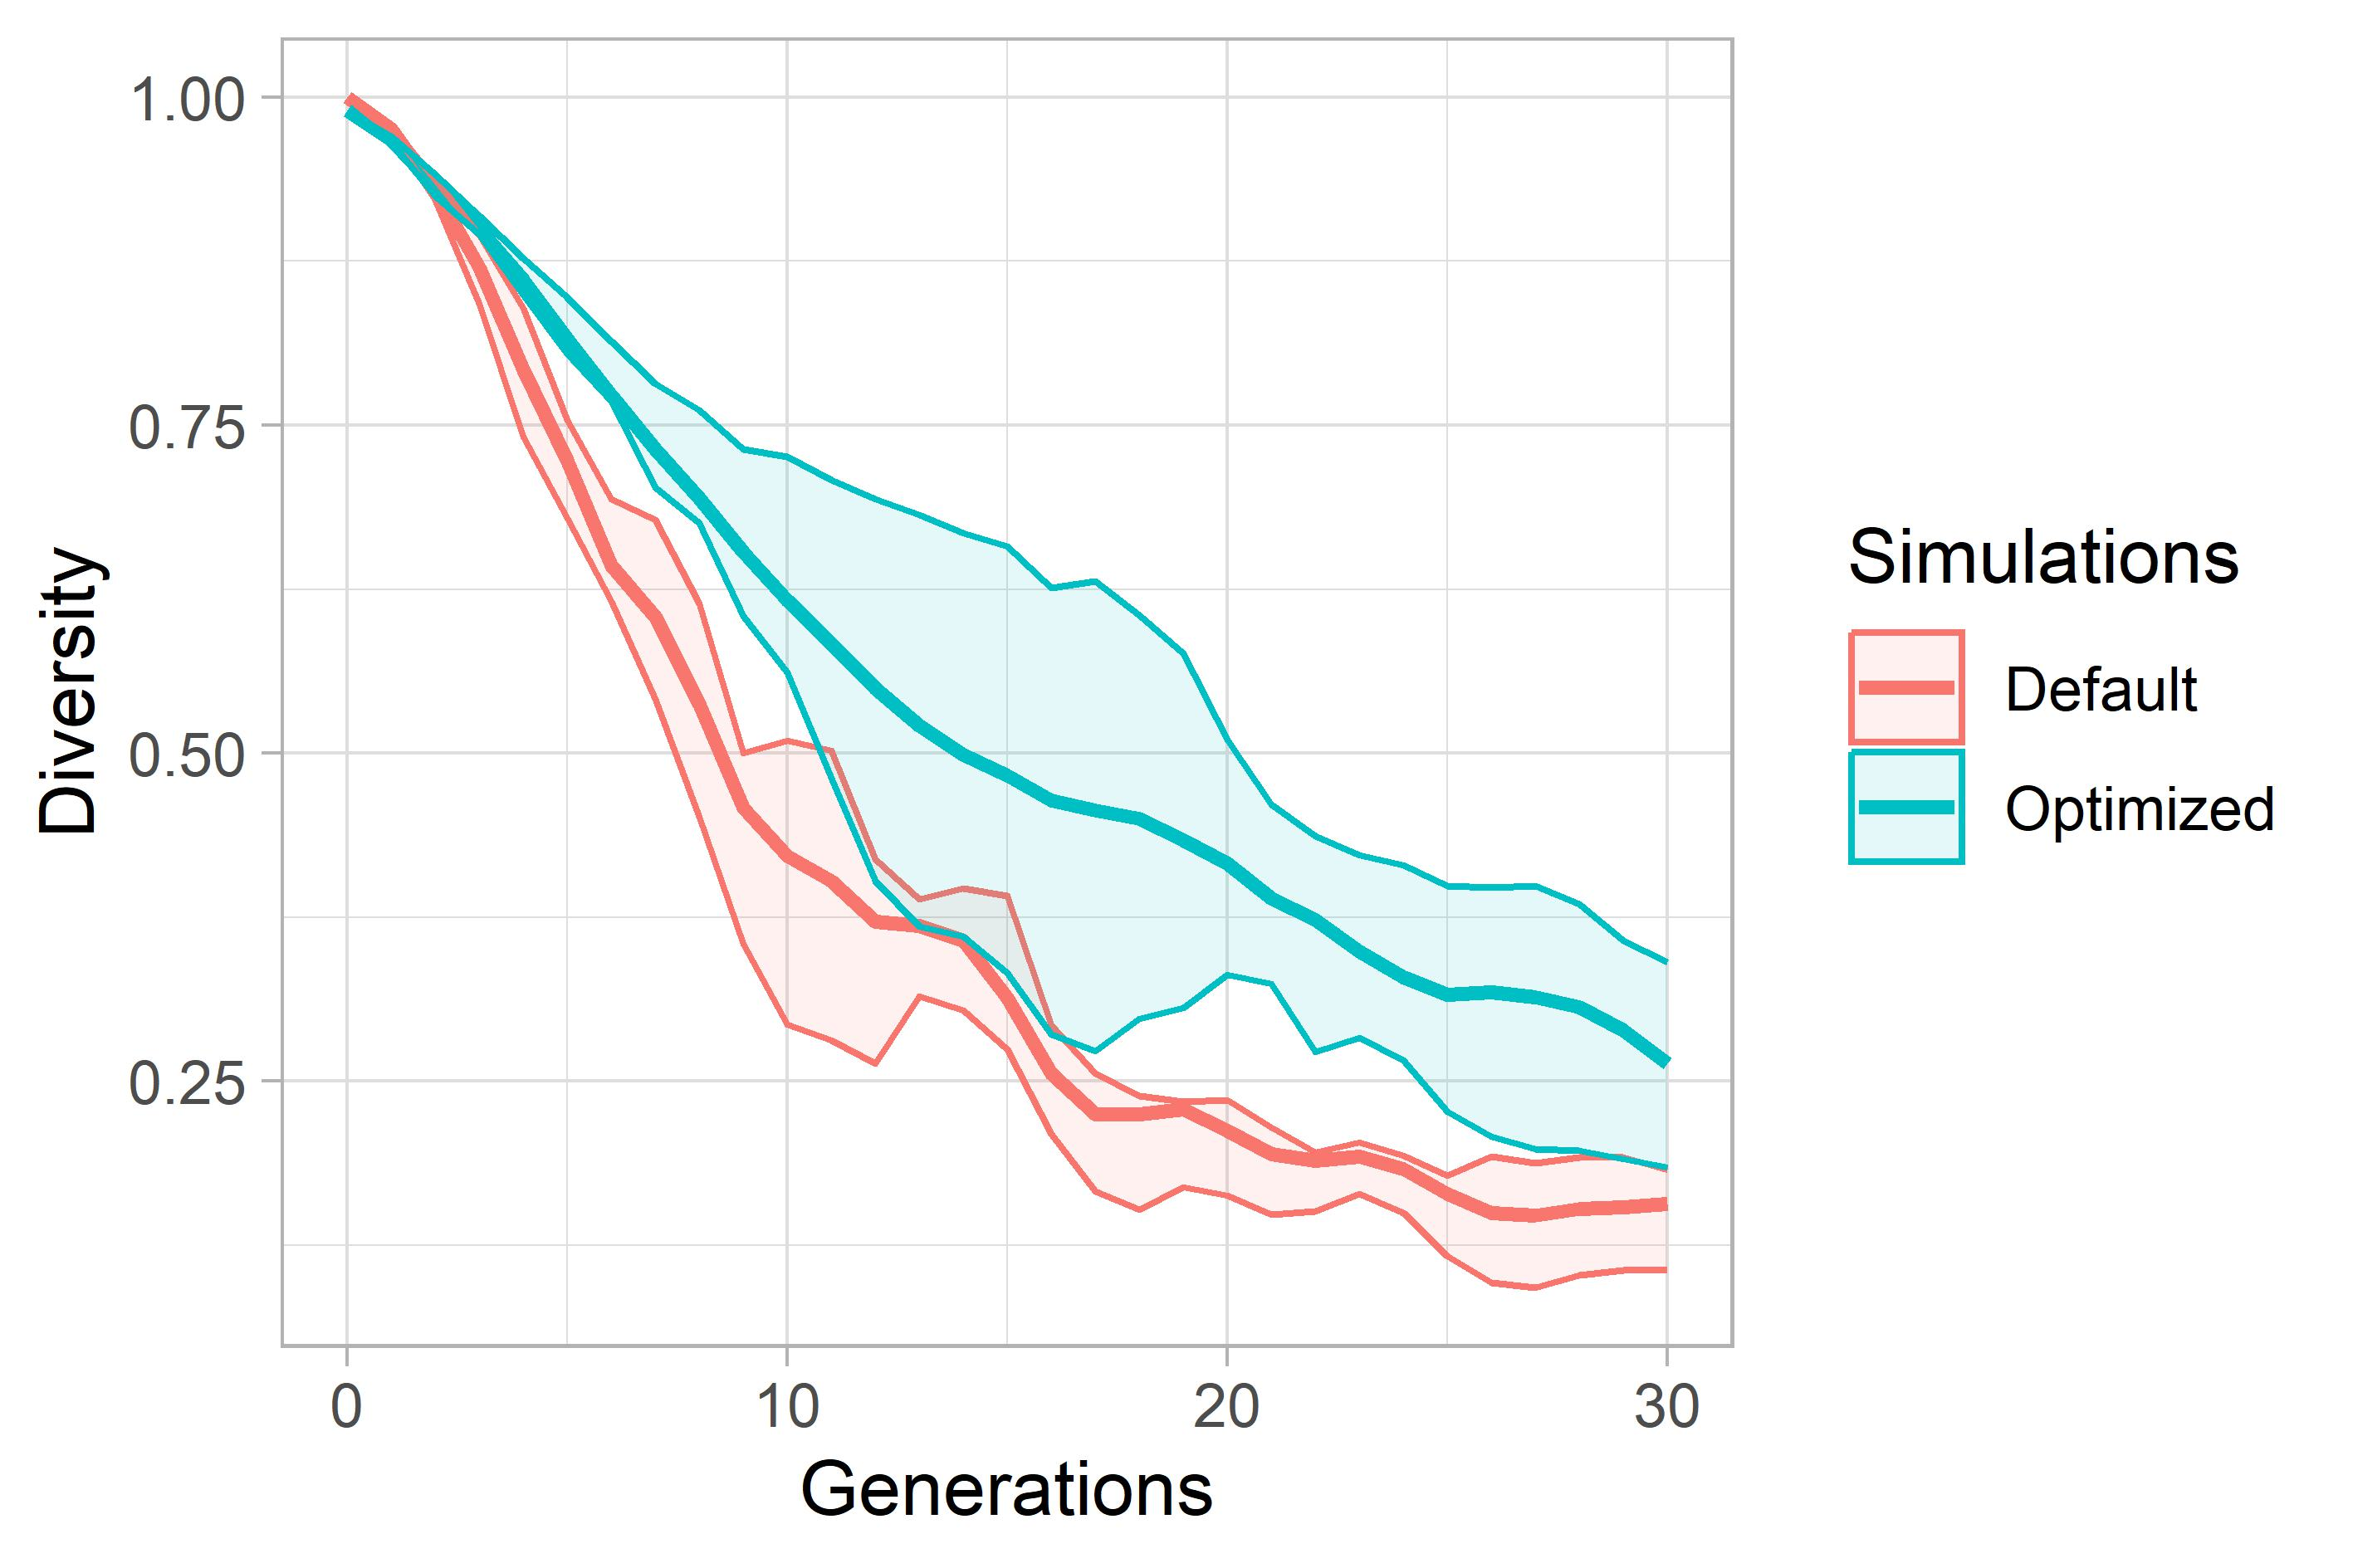
\includegraphics[width=1\linewidth]{simulations/evaluation/plots/sim_3_ga_diversity} 
	\end{minipage} 
	\caption{start scenario 3: comparison of GAs}
	\label{fig:evaluation:sim_3_ga_comparison}
\end{figure}


The rate of improved fitness of the Default GA drops very similar to the Optimized GA. The difference of decline in the diversity is also not as pronounced as in the previous two comparisons. While the optimized GA shows to still hold the diversity in the population longer, this only has a minimal impact on its average fitness. The similarity in performance might be explained by the smaller search space, which is a result of the reduced number of NPCs. Here, high mutation and crossover rates might not have the previously pronounced advantage.

\section{Start Scenario 4}
Start scenario 4 can be seen in Appendix at Figure \ref{fig:appendix:start_scenarios_3_4}. Eighteen vehicles with ten pedestrians are initialized, resulting in the start scenario with the most NPCs.

\begin{figure}[ht] 
	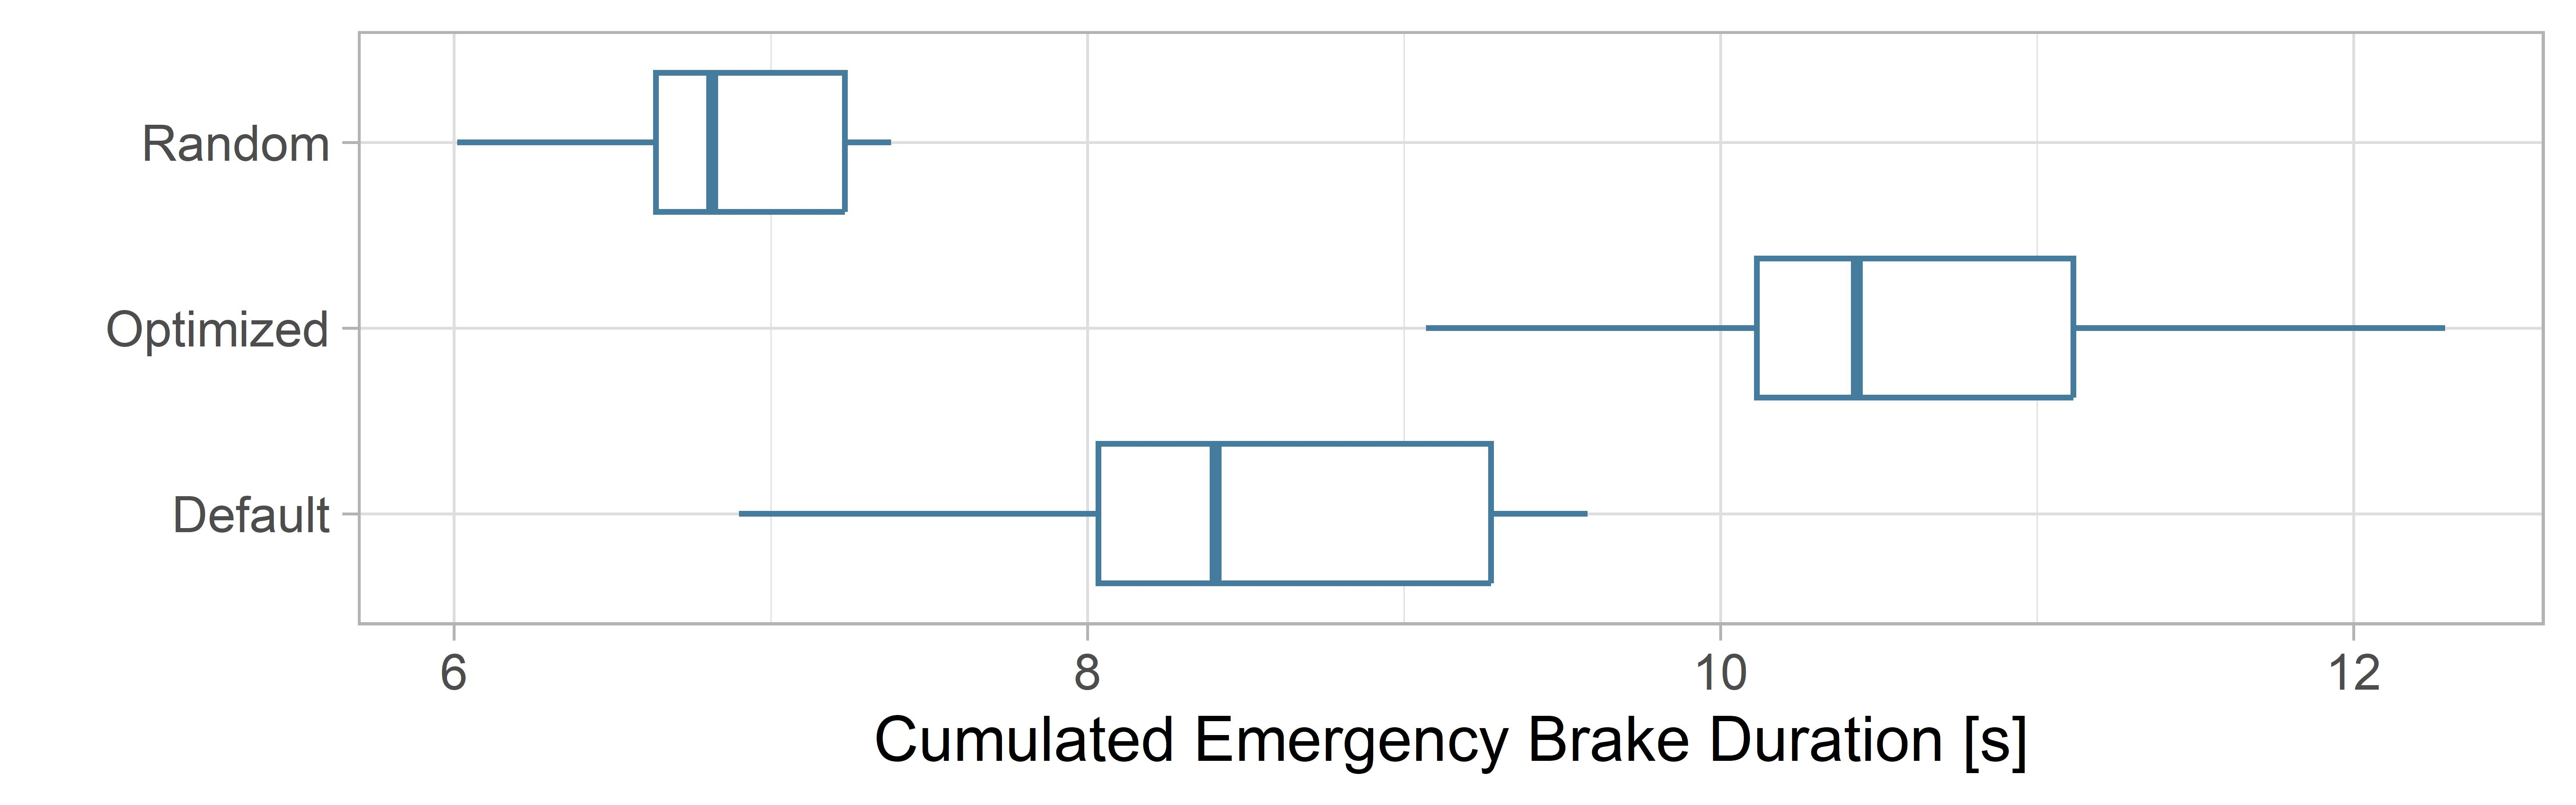
\includegraphics[width=1\linewidth]{simulations/evaluation/plots/sim_4_comparison}
	\caption{Start Scenario 4: Default GA vs Optimized GA vs Random Search}
	\label{fig:evaluation:sim_4_comparison}
\end{figure}

Figure \ref{fig:evaluation:sim_4_comparison} shows the Optimized GA clearly outperforming the Default GA as well as Random Search.
The Optimized GA (M = 10.60, SE = 0.29) has significantly greater fitness then the Default GA (M = 8.46, SE = 0.28) with \textit{t}(17.98) = 5.30, p < 0.001, and a large effect r = 0.78.
Compared to Random Search (M = 6.86, SE = 0.14), the greater fitness of the Optimized GAs is significant with \textit{t}(11.71) = 12.7, p < 0.001, and a large effect r = 0.96. Both genetic algorithms performance over the generations next to their diversity chart is compared in Figure \ref{fig:evaluation:sim_4_ga_comparison}.

\begin{figure}[ht] 
	\begin{minipage}[b]{0.5\linewidth}
		\centering
		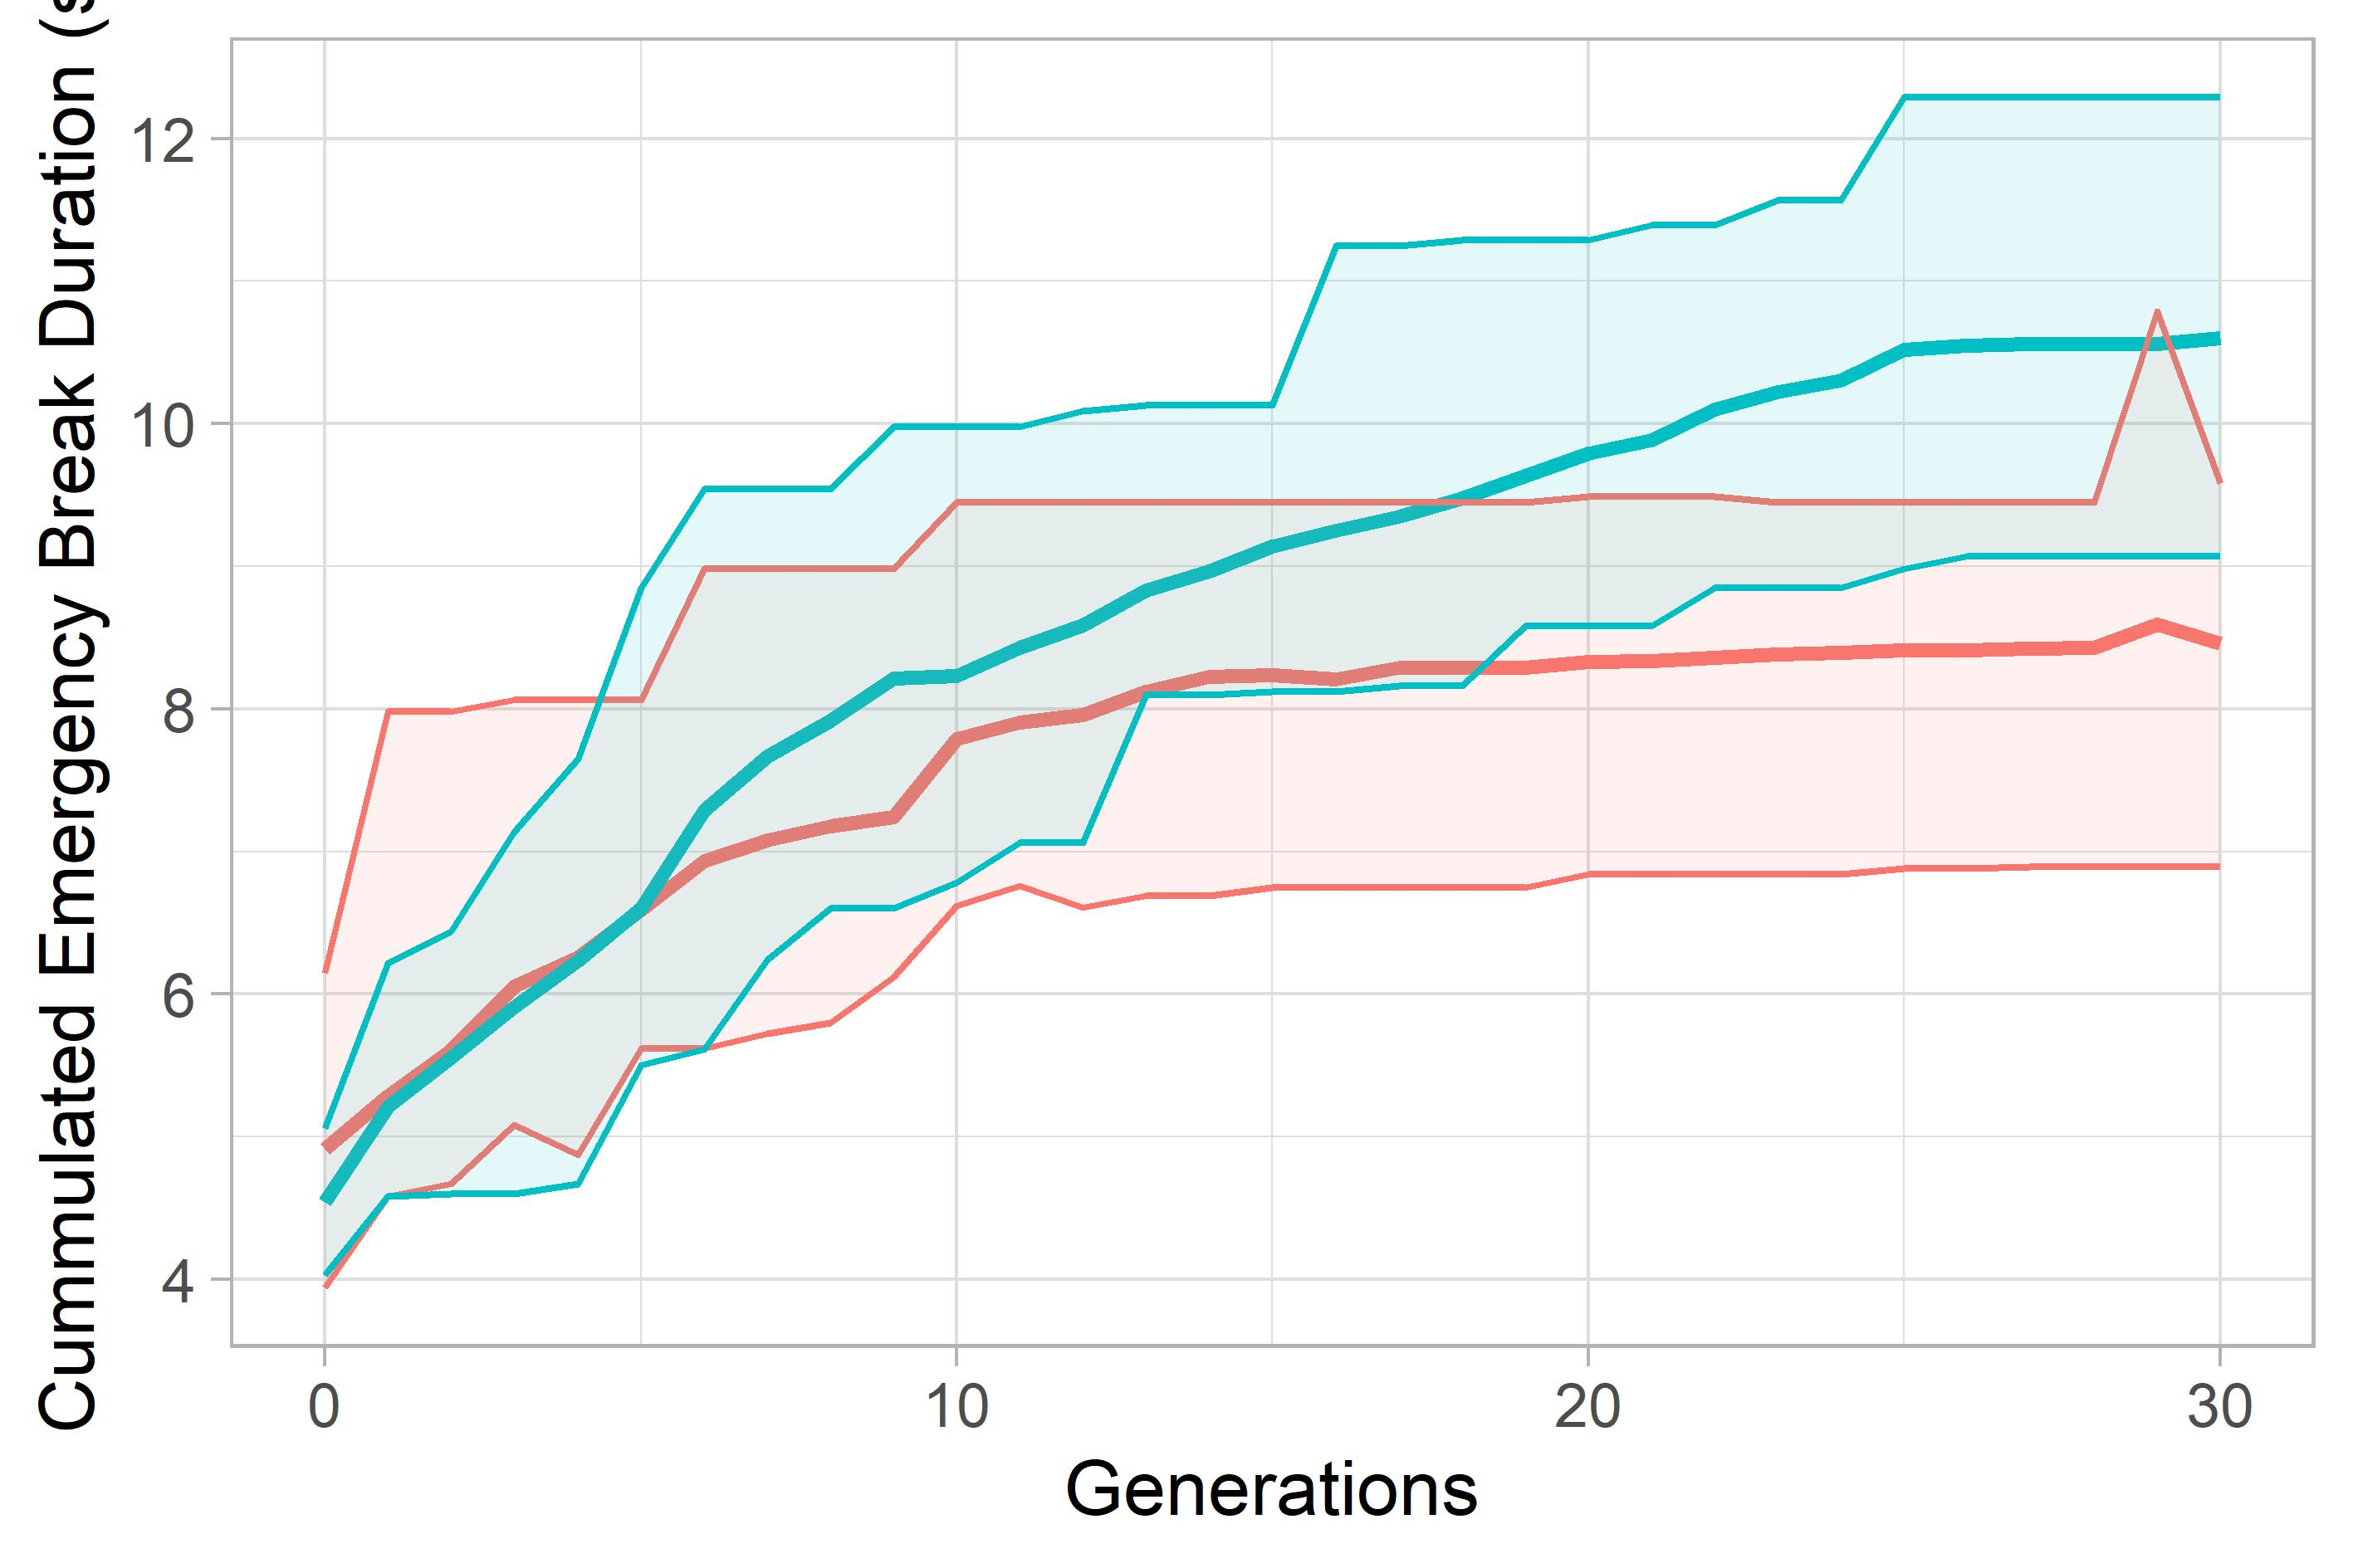
\includegraphics[width=1\linewidth]{simulations/evaluation/plots/sim_4_ga_generations} 
	\end{minipage}%%
	\begin{minipage}[b]{0.5\linewidth}
		\centering
		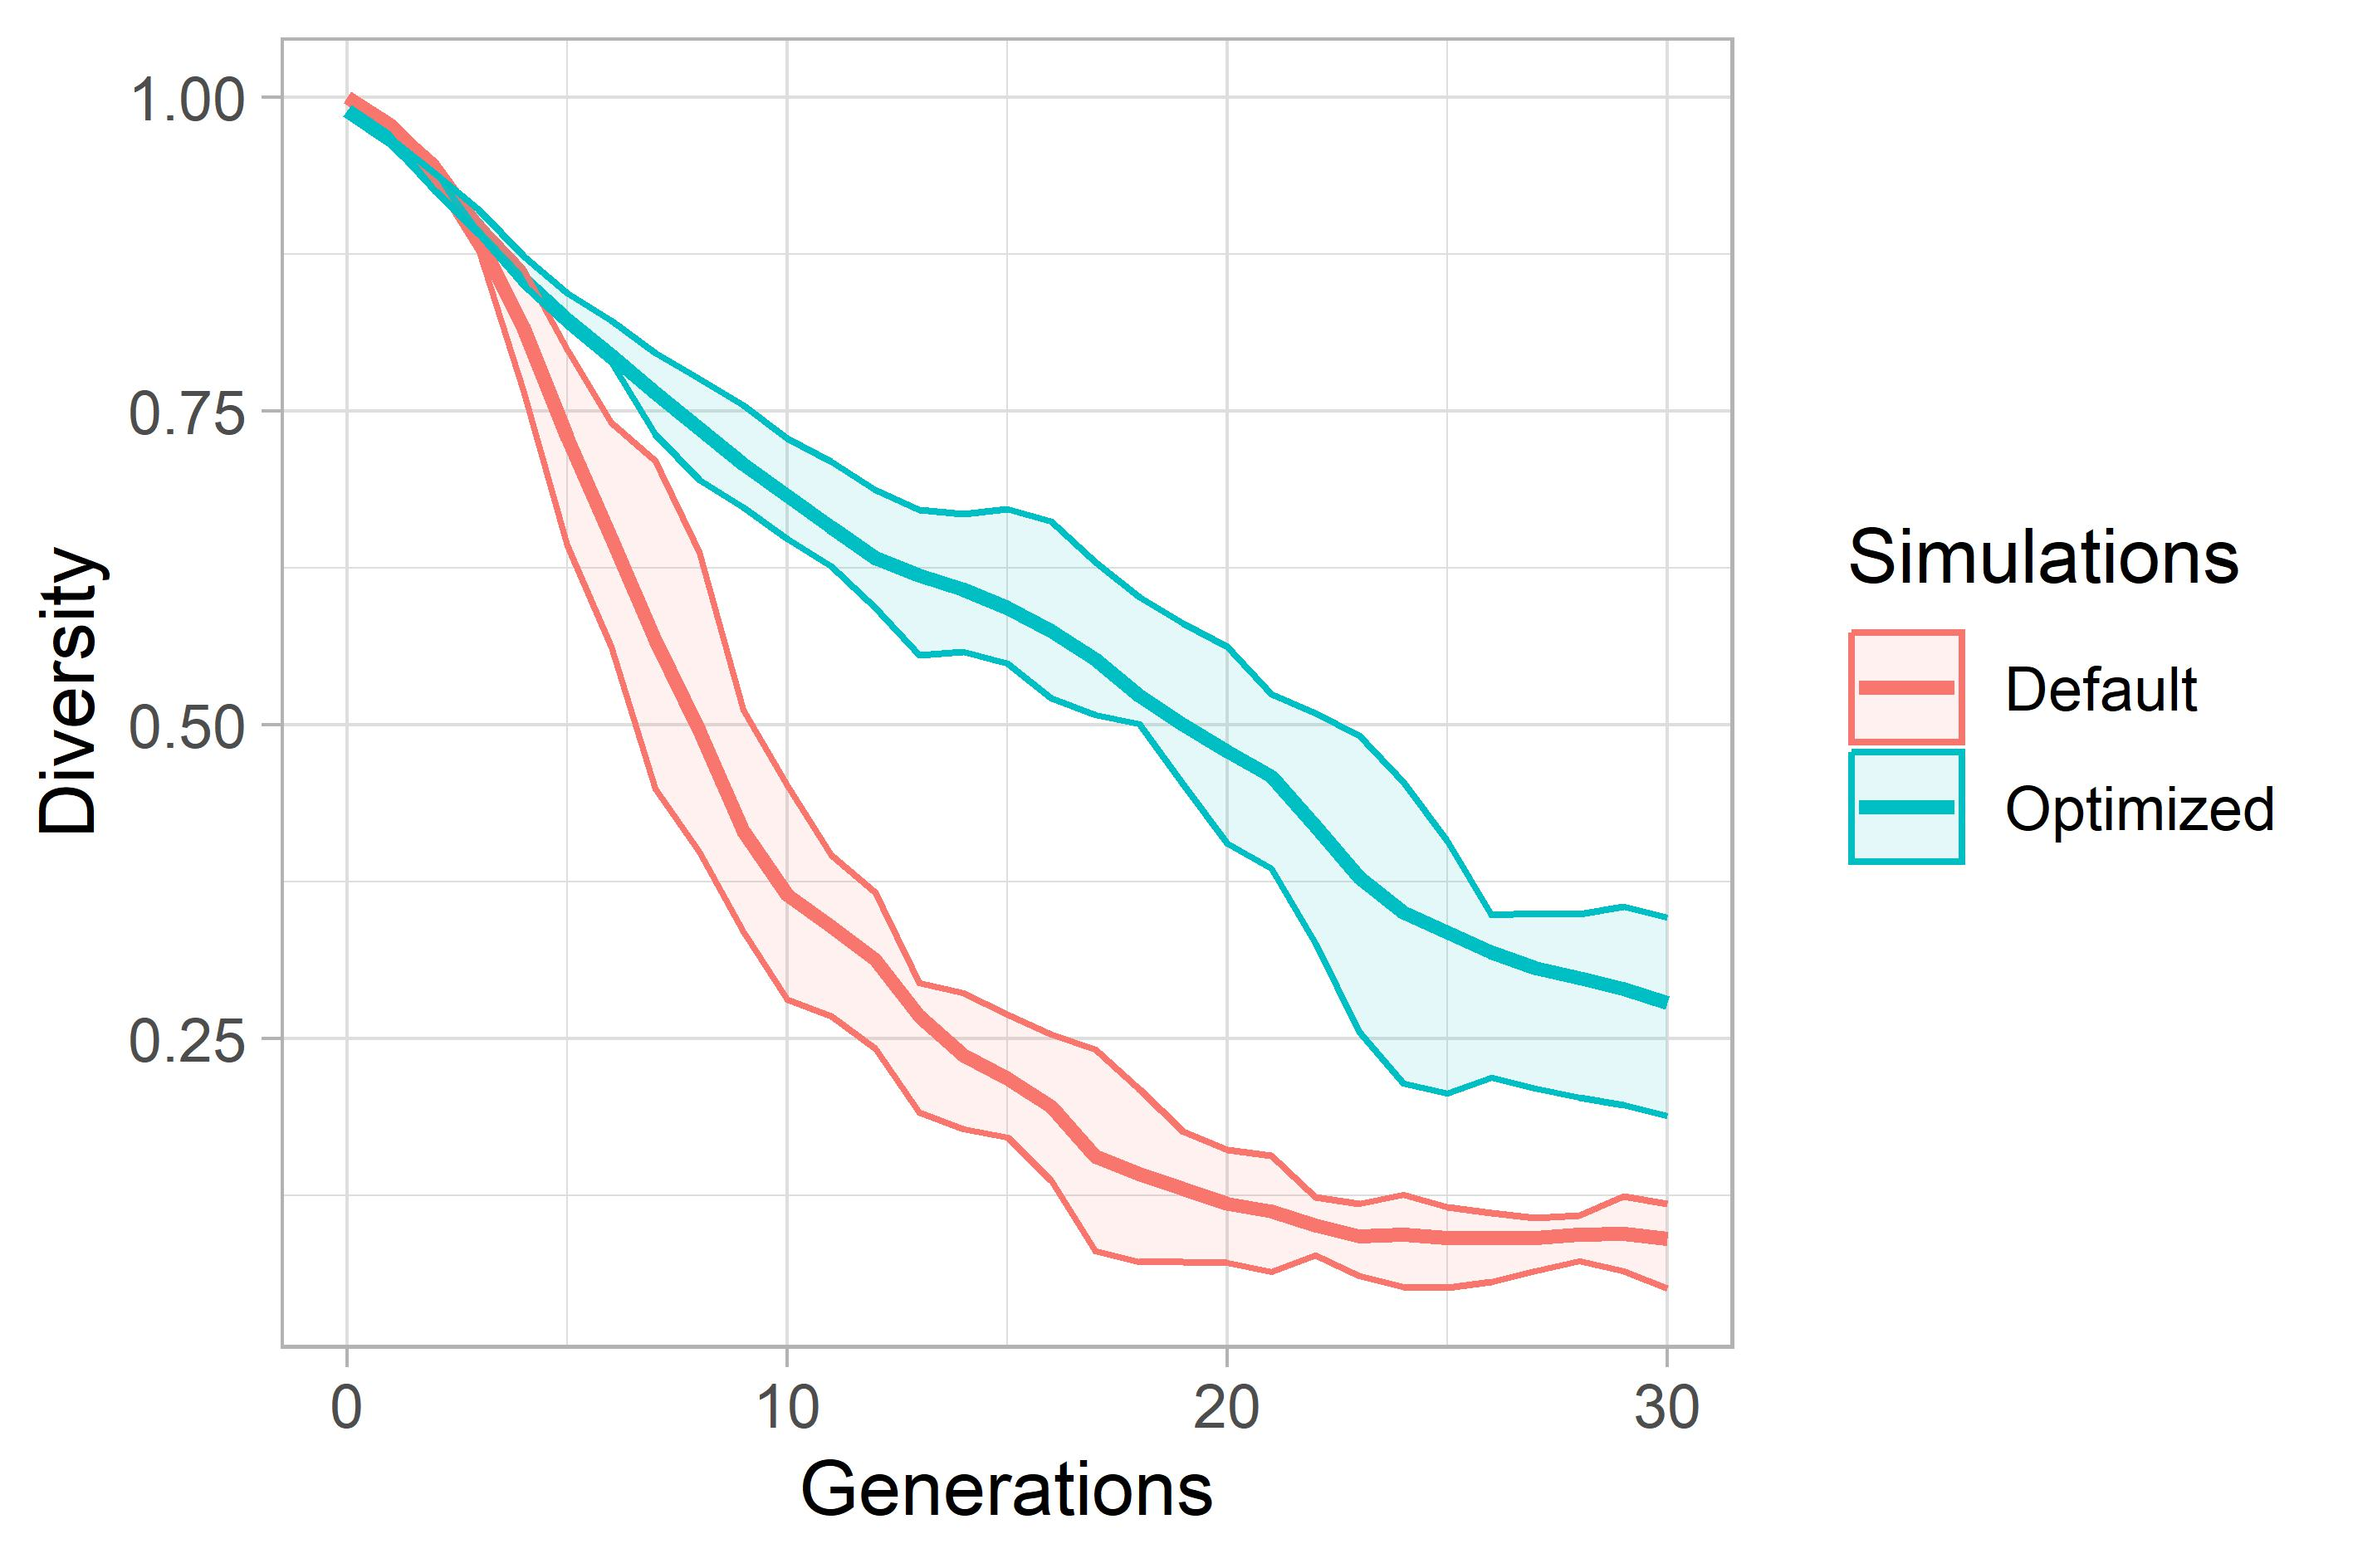
\includegraphics[width=1\linewidth]{simulations/evaluation/plots/sim_4_ga_diversity} 
	\end{minipage} 
	\caption{start scenario 4: comparison of GAs}
	\label{fig:evaluation:sim_4_ga_comparison}
\end{figure}

Already at generation 5, the average rate of improved fitness of the Default GA drops compared to the Optimized GA. This decline is accompanied by an early, sharp reduction in the diversity. In contrast, the optimized GA shows to be able to hold the diversity much longer at a high level, its rate of diversity drop is linear. The results underline the statement made in Section \ref{sect:evaluation:scenario_3}, asserting that the Optimized GA excels at scenarios with lots of NPCs, where a vast search space is given.



